%%%%%%%%%%%%%%%%%%%%%%%%%%%%%%%%%%%%%%%%%%%%%%%%%%%%%%%%%%%%%%%%%%%%%%%%%%%%%%
% ASU Dissertation Template
%%%%%%%%%%%%%%%%%%%%%%%%%%%%%%%%%%%%%%%%%%%%%%%%%%%%%%%%%%%%%%%%%%%%%%%%%%%%%%
% Copyright 2021 Robert W. Kutter (robert@kutterconsulting.com)
%
%   See also: http://kutterconsulting.com
%
% For guidance on using this file, see the README.
%
%%%%%%%%%%%%%%%%%%%%%%%%%%%%%%%%%%%%%%%%%%%%%%%%%%%%%%%%%%%%%%%%%%%%%%%%%%%%%%
% Preamble
%%%%%%%%%%%%%%%%%%%%%%%%%%%%%%%%%%%%%%%%%%%%%%%%%%%%%%%%%%%%%%%%%%%%%%%%%%%%%%
\newcommand*{\pointsize}{12pt}          %<Set the font size; make sure the size is correct
                                        %   for the font you will use
\documentclass[letterpaper,             % Use US letter-size paper
               oneside,                 % No verso and recto differences
               \pointsize]              % Uses the font size defined above
               {memoir}
\renewcommand{\cleardoublepage}%        % \cleardoublepage will create entirely blank
  {\clearpage}%                         %   pages depending on settings (e.g., usually
                                        %   before start of \mainmatter); redefine it here
                                        %   so that no entirely blank pages are created
                                        %   automatically
%%%%%%%%%%%%%%%%%%%%%%%%%%%%%%%%%%%%%%%
% (Some) Packages
%%%%%%%%%%%%%%%%%%%%%%%%%%%%%%%%%%%%%%%
\usepackage{graphicx}                   % For importing image files
\usepackage{etoolbox}                   % For advanced commands throughout preamble
\usepackage{microtype}                  %~Improves kerning and protrusion (optional);
                                        %   See here for an introduction:
                                        %   http://www.khirevich.com/latex/microtype/

\providetoggle{usemicrotype}            % TRUE = microtype is being used
\makeatletter                           %   (Used to turn of microtype protrusion in the
\@ifpackageloaded{microtype}%           %   table of contents.)
  {\settoggle{usemicrotype}{true}}%
  {\settoggle{usemicrotype}{false}}
\makeatother
\usepackage{changepage}                 % For changing page layout (e.g., margins) in the
                                        %   middle of the document
\usepackage{calc}					              % Calculate text widths; used in page layout
                                        %   changes

%%%%%%%%%%%%%%%%%%%%%%%%%%%%%%%%%%%%%%%
% Title page, input
%%%%%%%%%%%%%%%%%%%%%%%%%%%%%%%%%%%%%%%
\listadd{\titlelines}%
  {First Line of the Title}             %<Enter the title of the dissertation
\listadd{\titlelines}%
  {Second Line of the Title}            % If you want to
                                        %   split the title across lines,
                                        %   use another \listadd command for the
                                        %   second line
\newcommand*\Author{Your Name}          %<Enter your name; must match official transcript
\newcommand*{\documentname}%
  {Dissertation}                        %<Enter the type of document (capitalized)
\newcommand*{\degreename}
  {Doctor of Philosophy}                %<Enter the type of degree (capitalized)
\newcommand*\defdate{April 2021}        %<Give month (written out fully) and year of
                                        %   the oral defense
\listadd{\committeechair}{Chair Name}   %<Enter committee chair name; use \listadd for
%\listadd{\committeechair}{Another name}%   for additional names
\newcommand*{\chairlabel}{Chair}        %<If you have co-chairs, replace this text with
                                        %   'Co-Chair'
\listadd{\committeemember}{Member Name} %<Enter committee member names; use \listadd for
\listadd{\committeemember}{Member Name} %   additional names
\newcommand*{\gradmonth}{May}           %<Enter the graduation date; month can only be:
                                        %  May, August, or December
\newcommand*{\gradyear}{2021}           %<Enter the graduation year, e.g. 2014

\listadd{\keywords}{keyword 1}          %<Enter keywords; use \listadd for
\listadd{\keywords}{keyword 2}          %   additional names (up to 6)
\newcommand*{\graddate}{\gradmonth%     % Compose full graduation date
  \space\gradyear}

%%%%%%%%%%%%%%%%%%%%%%%%%%%%%%%%%%%%%%%
% Page layout
%%%%%%%%%%%%%%%%%%%%%%%%%%%%%%%%%%%%%%%
\settrimmedsize{\stockheight}%          % Specifies \paperheight and \paperwidth
  {\stockwidth}{*}
\settrims{0pt}{0pt}                     % Set location of page in relation to the stock.
                                        % Paper and stock size are equivalent,
                                        % so both \trimtop and \trimedge are set to 0pt
\newlength{\forfootskip}
\setlength{\forfootskip}%
  {3\baselineskip}
\newlength{\textblockheight}            % Calculate height of text block to leave room
\setlength{\textblockheight}{9.0in}     %   for footers, keeping page numbers outside
\addtolength{\textblockheight}%         %   the 1in vertical margins
  {-\forfootskip}
\settypeblocksize{\textblockheight}%    % Calculated by 1.0in vertical margins and
  {*}{*}                                %   letting margins set the width of the typeblock
\setulmargins{1.0in}{*}{*}              % Set upper margin (\uppermargin, not \topmargin);
                                        %   calculate the bottom margin
\setlrmarginsandblock{1.25in}{1.25in}{*}%~Set margins and calculate width of typeblock
\setheaderspaces{*}{0.5\baselineskip}{*}% Arguments: '\headdrop', '\headsep', and/or ratio
                                        %   Note: This is only used in the list of
                                        %   contents sections
\setheadfoot{\baselineskip}%            % Set '\headheight' and '\footskip'
  {\forfootskip}
\checkandfixthelayout                   % Required by memoir package after setting layout
\settypeoutlayoutunit{in}               % Write layout dimensions to log file in inches

%%%%%%%%%%%%%%%%%%%%%%%%%%%%%%%%%%%%%%%
% Fonts
%%%%%%%%%%%%%%%%%%%%%%%%%%%%%%%%%%%%%%%
\usepackage[T1]{fontenc}                % Standard option to handle, e.g., accented
                                        %   characters like 'ö' better
\usepackage{amssymb,mathtools}          % For AMS-LaTeX, see here for more:
                                        %     http://www.ams.org/publications/authors/tex/amslatex
                                        % ('mathtools' loads and extends 'amsmath')
\usepackage{ifxetex,ifluatex}           % Can check if XeTeX or LuaTeX was used to typeset
\usepackage{fixltx2e}                   % Provides \textsubscript
\IfFileExists{upquote.sty}%             % Use upquote if available, for
  {\usepackage{upquote}}{}              %   straight quotes in verbatim environments

% Load fonts depending on the
%   typesetting engine
\ifnum 0\ifxetex 1\fi\ifluatex 1\fi=0   % If pdftex
  \usepackage[utf8]{inputenc}           %   'utf8' should match the encoding of this file
                                        %
                                        %~Set up your font in pdftex here
                                        %
\else 									                % If xetex or luatex
  \ifxetex                              % If xetex
    \usepackage{mathspec}               % Matches non-math open-type font to math
                                        %   open-type font (use 'mathspec' if you want to
                                        %   write math in unicode)
    \usepackage{xunicode}               % Convert LaTeX character macros to unicode
  \else                                 % If luatex\usepackage{fontspec}
    \usepackage{fontspec}               % Use fontspec for (open type) font selection
  \fi
  \defaultfontfeatures{Mapping=tex-text,% Font spec setting
    Scale=MatchLowercase}
  \newcommand*{\euro}{€}

  % Using fonts in XeLaTeX can be complicated; the following settings
  % work when this file is compiled inside the Docker container produced
  % by the `build.sh` script.
  %
  % Sometimes something simple like the following will work:
  %
  %   \setmainfont{Garamond}
  %
  % But often the easiest solution is to move font files (*.otf or *.ttf) into
  % a sub-directory and provide the direct path to them here.
  %
  % See `fontspec` documentation for more on using local font files.
  %
  \setmainfont{EBGaramond12}[           %<Set the main font; make sure the font is correct
                                        %   for the font size (See ASU Style Guide)
    Path          = /usr/share/fonts/opentype/ebgaramond/,
    Extension     = .otf ,
    UprightFont   = *-Regular ,
    ItalicFont    = *-Italic ,
    % Notice that bold is missing here because the Docker image does not have
    % a bold typeface for Garamond; it would probably be possible to find
    % one on your local system or online.
  ]

%  \setmathfont(Digits,Latin,Greek)%     %~Uncomment two lines to set a font for math%
%    {MATHFONT}
\fi

%%%%%%%%%%%%%%%%%%%%%%%%%%%%%%%%%%%%%%%
% Line spacing
%%%%%%%%%%%%%%%%%%%%%%%%%%%%%%%%%%%%%%%
\DoubleSpacing                          % True double spacing
\BeforeBeginEnvironment{quote}          % Memoir leaves most special material
  {\par\SingleSpacing}                  %   single spaced, but makes block quotes
\AfterEndEnvironment{quote}%            %   double-spaced; fix to follow ASU style guide
  {\vspace{-\baselineskip} %
  \DoubleSpacing}
\BeforeBeginEnvironment{quotation}%
  {\par\SingleSpacing}
\AfterEndEnvironment{quotation}%
  {\vspace{-\baselineskip} %
  \DoubleSpacing}

\setlength{\footnotesep}{\baselineskip} % Double space *between* footnotes
\renewcommand*{\footnoterule}{%         % Redefine footnoterule so that initial footnote
  \kern-3pt%                            %   still appears right under the rule (changing
  \hrule width 0.4\columnwidth          %   \footnotesep also changes the space between the
  \kern 2.6pt                           %   rule and the first footnote
  \vspace{-0.5\baselineskip}            % (Here is the vertical space adjustment)
  }

\usepackage{enumitem}                   % Control spacing in enumerate environment
\setlist{noitemsep}                     % Remove extra vertical spacing between items in lists
                                        % \setlist{nosep} to leave no space around whole list

%%%%%%%%%%%%%%%%%%%%%%%%%%%%%%%%%%%%%%%
% Page numbering
%%%%%%%%%%%%%%%%%%%%%%%%%%%%%%%%%%%%%%%
\makepagestyle{ASU}
  \makeevenfoot{ASU}{}{\thepage}{}
  \makeoddfoot{ASU}{}{\thepage}{}

%%%%%%%%%%%%%%%%%%%%%%%%%%%%%%%%%%%%%%%
% Title page, formatting
%%%%%%%%%%%%%%%%%%%%%%%%%%%%%%%%%%%%%%%
\newlength{\savedfootskip}
\setlength{\savedfootskip}{\footskip}
\newcommand{\titlepagesetup}{%          % Page layout for title page
  \changepage%                          % Adjustment to page dimensions:
    {\savedfootskip}%                   %   text height
    {}%                                 %   text width
    {}%                                 %   even-side margin
    {}%                                 %   odd-side margin
    {}%                                 %   column sep.
    {}%                                 %   topmargin
    {}%                                 %   headheight
    {}%                                 %   headsep
    {-\savedfootskip}%                  %   footskip
}

\newcommand{\closetitlepagesetup}{%     % Undo set up for title page
  \changepage{-\savedfootskip}{}{}{}{}%
    {}{}{}{\savedfootskip}%
}

\makeatletter                           % Do not modify this section; Enter info above
\newcommand*{\titlepageASU}{
  \titlepagesetup
  \clearpage
  \begin{center}
  \SingleSpacing
  \thispagestyle{empty}
    \renewcommand*{\do}[1]{##1 \\[\baselineskip]}
    \dolistloop{\titlelines}
    by \\[\baselineskip]
    \Author \\[5\baselineskip]
    A \documentname~Presented in Partial Fulfillment \\
    of the Requirements for the Degree \\
    \degreename \\
    \vfill                              % Vertically center the portion below
    Approved \defdate~by the \\
    Graduate Supervisory Committee: \\[\baselineskip]
    \renewcommand*{\do}[1]{##1, \chairlabel \\}
    \dolistloop{\committeechair}
    \renewcommand*{\do}[1]{##1 \\}
    \dolistloop{\committeemember}
    \vfill                              % Vertically center the portion above
    ARIZONA STATE UNIVERSITY \\[\baselineskip]
    \graddate
  \end{center}
  \clearpage
  \closetitlepagesetup
}
\makeatother

%%%%%%%%%%%%%%%%%%%%%%%%%%%%%%%%%%%%%%%
% Heading styles
%%%%%%%%%%%%%%%%%%%%%%%%%%%%%%%%%%%%%%%
% Note: memoir also has \book and \part commands; do not use these
\makechapterstyle{ASU}{%                % Define chapter heading style
  \renewcommand*{\chapterheadstart}{}   % Chapter title flush with top margin
  \renewcommand*{\chapnamefont}%        % Set font for 'Chapter' or 'Appendix'
    {\normalfont}
  \renewcommand*{\chapnumfont}%         % Set font for number in chapter headings
    {\normalfont}
  \renewcommand*{\afterchapternum}%     % Insert a double line break after
    {\\[\baselineskip]}                 %   chapter number
  \renewcommand*{\chaptitlefont}%       % Set font for chapter title name
    {\normalfont}
  \setlength{\afterchapskip}{0pt}       % Set vertical space between chapter title and
                                        %   first paragraph; equivalent to one line break
                                        %   (vertical space = \afterchapskip + \baselineskip)
                                        % Note: This \afterchapskip value is only used in
                                        %   front matter
  \renewcommand*{\printchapternum}{%    % Center justify chapter number
    \centering \chapnumfont %
    \thechapter}
  \renewcommand*{\printchaptertitle}[1]%% Center justify
    {\expandafter\centering %           %   \MakeUppercase has issues; see here for some
    \expandafter\chaptitlefont %        %   details: https://tex.stackexchange.com/questions/35680/uppercase-in-newcommand
    \expandafter\MakeUppercase %        %   Accented characters and some fonts may not
    \expandafter{##1}}                  %   uppercase correctly; if that happens, just
                                        %   type the chapter title in uppercase
}

\setsecnumdepth{all}                    %~Enter the levels that you want to have numbered
                                        %   (Default is to number all [5 levels deep].)

\newcommand{\divisionbeforeskip}%       % Create default formatting for headings
  {\baselineskip}
\newcommand{\divisionindent}%
  {0.5em}
\newcommand{\divisionfont}{\normalfont} % Font must be \normalfont
\newcommand{\divisionafterskip}%
  {\baselineskip}

\setbeforesecskip{\divisionbeforeskip}  % Apply default formatting to all heading levels
\setsecindent{\divisionindent}          % Note: If you change \setsecnumdepth above, you
\setsecheadstyle{\divisionfont}         %   will need to set the indent for all lower
\setaftersecskip{\divisionafterskip}    %   levels to '0pt'; otherwise, they will be
                                        %   preceded by unnecessary space
\setbeforesubsecskip{\divisionbeforeskip}
\setsubsecindent{\divisionindent}
\setsubsecheadstyle{\divisionfont}
\setaftersubsecskip{\divisionafterskip}

\setbeforesubsubsecskip{\divisionbeforeskip}
\setsubsubsecindent{\divisionindent}
\setsubsubsecheadstyle{\divisionfont}
\setaftersubsubsecskip{\divisionafterskip}

\setbeforeparaskip{\divisionbeforeskip}
\setparaindent{\divisionindent}
\setparaheadstyle{\divisionfont}
\setafterparaskip{\divisionafterskip}

\setbeforesubparaskip{\divisionbeforeskip}
\setsubparaindent{\divisionindent}
\setsubparaheadstyle{\divisionfont}
\setaftersubparaskip{\divisionafterskip}

%%%%%%%%%%%%%%%%%%%%%%%%%%%%%%%%%%%%%%%
% Paragraph formatting
%%%%%%%%%%%%%%%%%%%%%%%%%%%%%%%%%%%%%%%
%\sloppybottom                          % Reduce the chances of widows
\raggedbottom                           % Loosens vertical spacing requirements, so
                                        %   \sloppybottom doesn't make pages look bad;
                                        %   it also prevents large gaps in the middle of
                                        %   pages and pushes them to the bottom of pages
\indentafterchapter                     % Overrides the default which is not to indent
                                        %   the first paragraph in a chapter, but it
                                        %   looks odd in some places to not indent
                                        %   paragraphs

%%% List Titles %%%
\renewcommand{\contentsname}%           % Set heading for each list
  {Table of Contents}%                  %   Formatted as chapter headings by default, so
\renewcommand{\listtablename}%          %   no additional heading formatting is needed
  {List of Tables}
\renewcommand{\listfigurename}%
  {List of Figures}

%%% Depth %%%
\settocdepth{subparagraph}              % Include 5 levels deep (all levels) in TOC

%%% Fonts %%%
\makeatletter%
\patchcmd{\l@part}%                     % Patch the command that writes part-level entries
    {\cftpartfont {#1}}%                %   to the table of contents, so they are in
    {\normalfont \texorpdfstring{%      %   'normalfont' and uppercase
      \uppercase{#1}}{{#1}} }%
    {\typeout{Success: Patch %
      'l@part' to uppercase %
      part-level headings in the %
      table of contents.}}%
    {\typeout{Fail: Patch %
      'l@part' to uppercase %
      part-level headings in the %
      table of contents.}}%
\makeatother%

\makeatletter%
\patchcmd{\l@chapapp}%                  % Patch the command that writes chapter-level
    {\cftchapterfont {#1}}%             %   entries to the table of contents, so they are
    {\normalfont \texorpdfstring{%      %   in 'normalfont' and uppercase
      \uppercase{#1}}{{#1}} }%
    {\typeout{Success: Patch %
      'l@chapapp' to uppercase %
      part-level headings in the %
      table of contents.}}%
    {\typeout{Fail: Patch %
      'l@chapapp' to uppercase %
      part-level headings in the %
      table of contents.}}%
\makeatother%

% If not using 'hyperref', use the following commands to adjust 'part' and 'chapter'
%   level headings in the TOC
%\renewcommand*{\cftpartfont}%          % Uppercase 'part' and 'chapter' headings
%  {\normalfont\MakeTextUppercase}      % Note: Sending \MakeTextUppercase to the TOC
%\renewcommand*{\cftchapterfont}%       %   conflicts with hyperref and breaks it!
%  {\normalfont\MakeTextUppercase}%

\usepackage{titlecaps}                  % Set up headline style for captions in the
                                        %   lists of tables and figures
                                        % Note: ASU style guide does not provide
                                        %   comprehensive guidelines for headlines, so
                                        %   Chicago style for headline style is used
                                        % Note: Last word in title is not explicitly
                                        %   capitalized; in general, these settings are
                                        %   broadly correct, but captions should be
                                        %   reviewed to ensure they are being capitalized
                                        %   properly
\Resetlcwords
\Addlcwords{a an the}                   % Leave articles lowercase
\Addlcwords{and but for or nor}         % Leave conjunctions lowercase
\Addlcwords{aboard about above across % % Leave all prepositions lowercase
  after against along amid among anti % %   (This is a [non-exhaustive] list of common
  around as at before behind below %    %   one-word prepositions)
  beneath beside besides between %
  beyond but by concerning considering %
  despite down during except excepting %
  excluding following for from in %
  inside into like minus near of off %
  on onto opposite outside over past %
  per plus regarding round save since %
  than through to toward towards under %
  underneath unlike until up upon %
  versus vs via with within without}
\Addlcwords{ according\space{to} %      % Leave two-word conjunctions lowercase
  ahead\space{of} apart\space{from} %   %   (This is a [non-exhaustive] list of common
  as\space{for} as\space{of} %          %   two-word prepositions.)
  as\space{per} as\space{regards} %
  aside\space{from} astern\space{of} %
  back\space{to} because\space{of} %
  close\space{to} due\space{to} %
  except\space{for} far\space{from} %
  in\space{to} inside\space{of} %
  instead\space{of} left\space{of} %
  near\space{to} next\space{to} %
  on\space{to} opposite\space{of} %
  opposite\space{to} out\space{from} %
  out\space{of} outside\space{of} %
  owing\space{to} prior\space{to} %
  pursuant\space{to} rather\space{than} %
  regardless\space{of} right\space{of} %
  subsequent\space{to} such\space{as} %
  thanks\space{to} that\space{of} %
  up\space{to}}

\renewcommand{\cfttableaftersnumb}%     % Put table captions in List of Tables in title
  {\titlecap}%                          %   case
\renewcommand{\cftfigureaftersnumb}%    % Put table captions in List of Figures in title
  {\titlecap}%                          %   case

\renewcommand*{\cftpartpagefont}%       % Use normal font for all page numbers
  {\normalfont}
\renewcommand*{\cftchapterpagefont}%
  {\normalfont}
\renewcommand*{\cftsectionpagefont}%
  {\normalfont}
\renewcommand*{\cftsubsectionpagefont}%
  {\normalfont}
\renewcommand*{\cftsubsubsectionpagefont}%
  {\normalfont}
\renewcommand*{\cftsubsubsectionpagefont}%
  {\normalfont}
\renewcommand*{\cftparagraphpagefont}%
  {\normalfont}
\renewcommand*{\cftsubparagraphpagefont}%
  {\normalfont}
\renewcommand*{\cftfigurepagefont}%
  {\normalfont}
\renewcommand*{\cfttablepagefont}%
  {\normalfont}

\cftpagenumbersoff{part}                % Turn off page numbers for 'part's, which are
                                        %   actually serving as headings within the TOC

%%% Vertical Space %%%
\setlength{\cftbeforepartskip}{0pt}     % Remove all additional vertical spacing so TOC
\setlength{\cftbeforechapterskip}{0pt}  %   is double spaced uniformly
\setlength{\cftbeforesectionskip}{0pt}
\setlength{\cftbeforesubsectionskip}{0pt}
\setlength{\cftbeforesubsubsectionskip}{0pt}
\setlength{\cftbeforeparagraphskip}{0pt}
\setlength{\cftbeforesubparagraphskip}{0pt}
\setlength{\cftbeforefigureskip}{0pt}
\setlength{\cftbeforetableskip}{0pt}

\renewcommand{\insertchapterspace}{%    % By default, extra vertical space (10pt) is
  \addtocontents{lof}%                  %   inserted between tables and figures from
    {\protect\addvspace{0pt}}%          %   different chapters; remove this extra space.
  \addtocontents{lot}%
    {\protect\addvspace{0pt}}%
}

%%% Horizontal Space %%%
\newlength{\levelindentincrement}       % Set indent to increase by the same amount for
\setlength{\levelindentincrement}{2em}  %   each level in the TOC; don't adjust figure
\newlength{\levelindent}                %   or table indents
\setlength{\levelindent}%
  {\levelindentincrement}
\setlength{\cftchapterindent}%
  {\levelindent}
\addtolength{\levelindent}%
  {\levelindentincrement}
\setlength{\cftsectionindent}%
  {\levelindent}
\addtolength{\levelindent}%
  {\levelindentincrement}
\setlength{\cftsubsectionindent}%
  {\levelindent}
\addtolength{\levelindent}%
  {\levelindentincrement}
\setlength{\cftsubsubsectionindent}%
  {\levelindent}
\addtolength{\levelindent}%
  {\levelindentincrement}
\setlength{\cftparagraphindent}%
  {\levelindent}
\addtolength{\levelindent}%
  {\levelindentincrement}
\setlength{\cftsubparagraphindent}%
  {\levelindent}
\addtolength{\levelindent}%
  {\levelindentincrement}

\setlength{\cftchapternumwidth}%        % Decrease space between number and heading for
  {0.85\cftchapternumwidth}             %   all heading levels
\setlength{\cftsectionnumwidth}%
  {0.85\cftsectionnumwidth}
\setlength{\cftsubsectionnumwidth}%
  {0.85\cftsubsectionnumwidth}
\setlength{\cftsubsubsectionnumwidth}%
  {0.85\cftsubsubsectionnumwidth}
\setlength{\cftparagraphnumwidth}%
  {0.85\cftparagraphnumwidth}
\setlength{\cftsubparagraphnumwidth}%
  {0.85\cftsubparagraphnumwidth}

% Calculate the indent to the first
% character in table and figure
% captions.
% This is more complicated because the
% document automatically considers
% the total number of figures and
% tables and increases the indent to
% make room for longer numbers.
\newcounter{totfigures}                 % Collect the total number of figures
\newcounter{tottables}                  % Collect the total number of tables

\providecommand\totfig{}                % Retrieve the total number of figures
\providecommand\tottab{}                % Retrieve the total number of tables

\makeatletter
\AtEndDocument{%                        % Store the totals
  \addtocounter{totfigures}{%
    \value{figure}%
  }%
  \addtocounter{tottables}{%
    \value{table}%
  }%
  \immediate\write\@mainaux{%
    \string\gdef\string\totfig{%
      \number\value{totfigures}%
    }%
    \string\gdef\string\tottab{%
      \number\value{tottables}%
    }%
  }%
}
\makeatother

% The calculation that appears inside
% this block needs to be done as the
% the document is written, not in the
% preamble. `\pretocmd` makes this
% calculation happen right before
% `\listoffigures` is executed.
\usepackage{calculator}
\pretocmd{\listoffigures}{%
  % Calculate the number of digits in
  % the total number of figures
  %
  % Here is the algorithm:
  %   Floor(Log10(\number)) + 1
  \MAX{\totfig}{1}{\figurecount}
  \LOG[10]{\figurecount}{\tempAfig}%
  \FLOOR{\tempAfig}{\tempBfig}%
  \ADD{\tempBfig}{1}{\digitsinfig}%     % Number of digits in number of figs
  %
  % Calculate space factor for figures
  % The space factor is just one less
  % than the number of digits, but it
  % must be at least 0.
  %
  \SUBTRACT{\digitsinfig}{1}{\tempDfig}%
  \MAX{\tempDfig}{0}{\tempEfig}%
  \MULTIPLY{\tempEfig}{0.55}{%
    \figspacefactor%                    % Space factor for figures in LOF
  }%
  % Apply the space factor for figures
  \setlength{\cftfigurenumwidth}{%      % Figure has the same 'level' as
    \cftchapternumwidth%                % 'chapter' in the figure list, so
  }%                                    % make the number spacing the same as
                                        % for chapters unless there are more
  \addtolength{\cftfigurenumwidth}{%    % than 9 figures; in that case, add
    \figspacefactor em%                 % extra space (as calculated in
  }%                                    % `\figspacefactor`
}{}{}

% Same space calculation for tables
\pretocmd{\listoftables}{%
  % Calculate the number of digits in
  % the total number of tables
  \MAX{\tottab}{1}{\tablecount}
  \LOG[10]{\tablecount}{\tempAtab}%
  \FLOOR{\tempAtab}{\tempBtab}%
  \ADD{\tempBtab}{1}{\digitsintab}%     % Number of digits in number of tabs
  % Calculate space factor for tables
  \SUBTRACT{\digitsintab}{1}{\tempDtab}%
  \MAX{\tempDtab}{0}{\tempEtab}%
  \MULTIPLY{\tempEtab}{0.55}{%
    \tabspacefactor%                    % Space factor for tables in LOT
  }%
  % Apply the space factor for tables
  \setlength{\cfttablenumwidth}{%
    \cftchapternumwidth%
  }%
  \addtolength{\cfttablenumwidth}{%
    \tabspacefactor em%
  }%
}{}{}

%%% Leaders/dots %%%
\renewcommand*{\cftdotsep}{1.7}         % Set distance between dots for all heading levels
\renewcommand*{\cftchapterleader}%      % Turn on dots for 'chapter' level
  {\normalfont\cftdotfill{\cftdotsep}}
\makeatletter                           % Bring leader dots over to page number (no gap)
  \renewcommand{\@pnumwidth}{1.55em}    %~Manually adjust
  \renewcommand{\@tocrmarg}{2.55em}
\makeatother

\renewcommand{\cfttableaftersnum}{.}    % Period after number in LOT
\renewcommand{\cftfigureaftersnum}{.}   % Period after number in LOF

%%% Printing List Titles and Headers in Content Lists
% Table of Contents (TOC)
\copypagestyle{ASUtoc}{ASU}%            % Page style for regular page in TOC
  \makeevenhead{ASUtoc}%
    {\leftmark}{}{Page}
  \makeoddhead{ASUtoc}%
    {\leftmark}{}{Page}

\copypagestyle{ASUtocFirst}{ASU}%       % Custom page headers for first page of TOC
  \makeevenhead{ASUtocFirst}%           %    (print out the title)
    {}%
    {\printchaptertitle{\contentsname}}%
    {}
  \makeoddhead{ASUtocFirst}%
    {}%
    {\printchaptertitle{\contentsname}}%
    {}

\renewcommand{\tocheadstart}{}%         % Usually content list titles are printed like
                                        %   chapter headings; empty that formatting

\renewcommand{\printtoctitle}[1]{}%     % Don't print TOC title using default method;
                                        %   it will be output in the header

\renewcommand{\aftertoctitle}{%         % On the first page of the TOC, print out the
  \thispagestyle{ASUtocFirst}%          %   TOC title using a custom page style and print
  \hfill Page\par%                      %   the heading for the page below in the regular
  }%                                    %   textbox
                                        % Note: Need '\par' before lists; see here: https://tex.stackexchange.com/questions/49882/yet-another-perhaps-a-missing-item-error

% List of Tables (LOT)
\copypagestyle{ASUlot}{ASU}%            % Page style for regular page in list of tables
  \makeevenhead{ASUlot}{Table}{}{Page}
  \makeoddhead{ASUlot}{Table}{}{Page}

\copypagestyle{ASUlotFirst}{ASU}%       % Custom page headers for first page of list of
  \makeevenhead{ASUlotFirst}%           %   tables (print out the title)
    {}%
    {\printchaptertitle{\listtablename}}%
    {}
  \makeoddhead{ASUlotFirst}%
    {}%
    {\printchaptertitle{\listtablename}}%
    {}

\renewcommand{\lotheadstart}{}%         % Usually content list titles are printed like
                                        %   chapter headings; empty that formatting;

\renewcommand{\printlottitle}[1]{}%     % Don't print LOT title using default method;
                                        %   it will be output in the header

\renewcommand{\afterlottitle}{%         % On the first page of the list of tables, print
  \thispagestyle{ASUlotFirst}%          %   out the title using a custom page style and
  Table\hfill Page\par}%                %   print heading below in regular textbox

% List of Figures (LOF)
\copypagestyle{ASUlof}{ASU}
  \makeevenhead{ASUlof}{Figure}{}{Page}
  \makeoddhead{ASUlof}{Figure}{}{Page}

\copypagestyle{ASUlofFirst}{ASU}%       % Custom page headers for first page of list of
  \makeevenhead{ASUlofFirst}%           %   figures (print out the title)
    {}%
    {\printchaptertitle{\listfigurename}}%
    {}
  \makeoddhead{ASUlofFirst}%
    {}%
    {\printchaptertitle{\listfigurename}}%
    {}

\renewcommand{\lofheadstart}{}%         % Usually content list titles are printed like
                                        %   chapter headings; empty that formatting

\renewcommand{\printloftitle}[1]{}%     % Don't print LOF title using default method;
                                        %   it will be output in the header

\renewcommand{\afterloftitle}{%         % On the first page of the list of figures, print
  \thispagestyle{ASUlofFirst}%          %   out the title using a custom page style and
  Figure\hfill Page\par}                %   print heading below in regular textbox

%%% Page layout (dimensions) for Contents Lists
\newlength{\verticalpush}               % Set up to change page dimensions for the table
                                        %   of contents
                                        % Push everything down so all the content is still
                                        %   1in from the top of the page, including the
                                        %   header, so the header is available for titles
                                        %   on the first page of contents lists and then
                                        %   the headings on subsequent pages
\setlength{\verticalpush}%              % Calculate difference between \headdrop and the
  {1.0in - \headdrop}                   %   total upper margin (1in), so you can push
                                        %   the top of the header down into the textbox

\newcommand{\contentslistsetup}{%       % Set up for contents lists
  \changepage%                          % Adjustment to page dimensions:
    {-\baselineskip}%                   %   text height
    {}%                                 %   text width
    {}%                                 %   even-side margin
    {}%                                 %   odd-side margin
    {}%                                 %   column sep.
    {\verticalpush}%                    %   topmargin
    {}%                                 %   headheight
    {}%                                 %   headsep
    {-\verticalpush+\baselineskip}%     %   footskip
}

\newcommand{\closecontentslistsetup}{%  % Undo set up for contents lists
  \changepage{\baselineskip}{}{}{}{}%
    {-\verticalpush}{}{}{\verticalpush-\baselineskip}%
}

% Content lists can also be output directly. If the following command were used, all the
%   headings would have to be output manually (i.e., can't rely on any memoir macros for
%   formatting or setting in contents lists headings and lists). It would be best to
%   create a custom macro, such as '\customtoc', to output headings and content lists
%   following the style guide.
%
% \makeatletter
%   \@starttoc{toc}
% \makeatother

% These pages partly explain why it's difficult to use 'afterpage' to change page layout
%   settings (essentially, it's because everything inside \afterpage has a local scope).
%   If it were possible to use 'afterpage' in that way, the content lists would  be
%   easier to format. A new page layout could be called after the first page of each
%   content  list. Instead, use page marks to get the layout required by the style guide.
% https://tex.stackexchange.com/questions/97126/attempts-to-manually-change-linewidth-ignored-by-latex
% https://tex.stackexchange.com/questions/85729/page-styles-only-work-for-thispagestyle-under-afterpage

%%%%%%%%%%%%%%%%%%%%%%%%%%%%%%%%%%%%%%%
% Footnotes and Endnotes
%%%%%%%%%%%%%%%%%%%%%%%%%%%%%%%%%%%%%%%
\usepackage{chngcntr}                   % Modify counters (e.g., for figures, footnotes)
\counterwithout*{footnote}{chapter}     % Make footnote numbering continuous throughout

\providetoggle{useendnotes}
\settoggle{useendnotes}{true}           %<Set to 'true' if you want to use endnotes
\iftoggle{useendnotes}{%                % Use the command \pagenote to create endnotes
                                        %   in the running text. They will be collected
                                        %   and printed in a 'Notes' section at the end
                                        %   of the document

  \makepagenote                         % Required in preamble if using endnotes
  \continuousnotenums                   % Numbering does *not* reset after each chapter
  \renewcommand*{\pagenotesubhead}[3]{} % No subheads inside note list (default is to
                                        %   divide them by chapter)
  \renewcommand*{\notenuminnotes}[1]%   % Remove extra space between note number and note
    {\normalfont #1.}                   %   text
  \renewcommand{\postnoteinnotes}%      % Double space *between* notes
    {\par\vspace{\baselineskip}}
}{}                                     % Do nothing here if not using endnotes

%%%%%%%%%%%%%%%%%%%%%%%%%%%%%%%%%%%%%%%
% Bibliography
%%%%%%%%%%%%%%%%%%%%%%%%%%%%%%%%%%%%%%%
\newcommand{\bibfilename}{%             %<Enter the name of the *.bib file containing the
  src/sample/library%                   %   reference information for sources cited in
}%                                      %   the text. God help you if you're doing
                                        %   citations manually.

\newcommand{\bibheading}{References}    %<Enter the heading for the references section:
                                        %   'References', 'Works Cited', or 'Bibliography'

\providetoggle{usebiblatex}             % True = a biblatex package is being used;
                                        %   False = 'natbib' is being used
\settoggle{usebiblatex}{true}           %~Set to 'false' to use 'natbib' intead of
                                        %   biblatex; I strongly recommend using biblatex
                                        %   because natbib is rather old and will break
                                        %   for innocuous things like underscores in URLs
\iftoggle{usebiblatex}{%                % Settings for citation package
%                                       % Settings for 'biblatex' or a version of
%                                       %   'biblatex'
  \usepackage[authordate,%
              backend=biber,%           % Recommend to use 'biber' instead of 'bibtex'
              doi=only,%                % Avoid printing URLs
              isbn=false]%              % Don't print ISBN numbers
              {biblatex-chicago}        %~Other possibilities include: 'biblatex',
                                        %   'biblatex-apa', and 'biblatex-mla'
  \bibliography{\bibfilename}
  \setlength{\bibitemsep}%              % Set vertical distance between
    {0.5\baselineskip}%                 %   bibliography entries
  \setcounter{biburlnumpenalty}{9000}   % Break URLs in bibliography across lines
  \setcounter{biburlucpenalty}{9000}
  \setcounter{biburllcpenalty}{9000}

  \usepackage[style=american,%          % Settings for quotation marks; load after
    english=american]{csquotes}%        %   'inputenc'; only use with biblatex; throws
  \MakeOuterQuote{"}%                   %   error when used with natbib
}{%                                     % Settings for 'natbib'
  \usepackage{natbib}%
  \newcommand{\natbibstyle}{%           %~Enter the name of the *.bst file to use to
    src/asudis%                         %   format citations with natbib. Default is
  }%                                    %   'asudis'. I do not know where 'asudis' came
                                        %   from, but apparently it formats citations
                                        %   correctly because it was included with the
                                        %   previous LaTeX template.
}

%%%%%%%%%%%%%%%%%%%%%%%%%%%%%%%%%%%%%%%
% Tables and figures
%%%%%%%%%%%%%%%%%%%%%%%%%%%%%%%%%%%%%%%
\captiondelim{. }                       %~Use period (.) after caption number instead of
                                        %   colon (:). Change according to style guide.
\captionstyle[\raggedright]%            % Set justifcation for [one line captions]
  {\raggedright}                        %   and {multiple line captions}
\setlength{\belowcaptionskip}{0pt}      % Bring caption down closer to figure/table
\makeatletter                           % Consecutive numbering throughout
  \counterwithout{figure}{chapter}      %   (including back matter)
  \counterwithout{table}{chapter}
  \renewcommand\@memfront@floats{}
  \renewcommand\@memmain@floats{}
  \renewcommand\@memback@floats{}
\makeatletter

\newcommand{\macrocapwrap}[1]{%         % Use this macro to place other macros inside
  {\bgroup\bgroup{{#1}}\egroup\egroup}% %   captions, e.g., '\macrocapwrap{\ref{figure1}}'
}%                                      % Note: Necessary due to the 'titlecaps' package
                                        %   which modifies contents of captions

%%% Tables %%%
%
% Note: 'memoir' natively supports commands from the following table-related packages:
%   tabularx, ccaption, booktabs.
% Everyone has particular ideas about how tables should look, so you may need to
%   load additional packages and modify the code below to get tables (and figures) to
%   look the way you want them to.
\setfloatadjustment{table}{\raggedright}% Left justify material inside table floats
\usepackage{tabu}                       % 'tabu' is an excellent table package; it can
                                        %   automatically size column widths and has a
                                        %   lot of customizations that other packages do
                                        %   not. It also has a 'longtabu' environment that
                                        %   emulates 'longtable' with additional features
                                        %   from the 'tabu' package. If you don't want
                                        %   to use it, you can comment this line out.
\BeforeBeginEnvironment{table}%         % Single space inside table environment
  {\SingleSpacing}
\AfterEndEnvironment{table}
  {\DoubleSpacing}

%%% Figures %%%
\setfloatadjustment{figure}%            % Left justify material inside figure floats
  {\raggedright}
\BeforeBeginEnvironment{figure}%        % Single space inside figure environment
  {\SingleSpacing}
\AfterEndEnvironment{figure}
  {\DoubleSpacing}

\makeatletter                           % Define custom macro called '\maxwidth{}' that
  \def\maxwidth#1{%                     %   allows you to specify the maximum width of an
    \ifdim%                             %   imported image. See below for an example.
      \Gin@nat@width>#1 #1%             %
    \else%                              % Source: http://tex.stackexchange.com/questions/86350/includegraphics-maximum-width
      \Gin@nat@width%
    \fi}
\makeatother
%
% Example \maxwidth:
%
%   \includegraphics[width=\maxwidth]{\textwidth}]{image.pdf}
%
% Note: This will keep an image inside the horizontal margins assuming the image starts
%   on the right margin (i.e., no horizontal space before the image).

%%%%%%%%%%%%%%%%%%%%%%%%%%%%%%%%%%%%%%%
% Hyperref settings
%%%%%%%%%%%%%%%%%%%%%%%%%%%%%%%%%%%%%%%

%%% URL Settings %%%
\PassOptionsToPackage{hyphens}{url}
\usepackage[breaklinks=true]{hyperref}  % 'hyperref' should be loaded at the end of the
                                        %   preamble; Note: the uppercasing commands used
                                        %   throughout the preamble can conflict with it,
                                        %   especially when non-standard fonts or
                                        %   different file encodings are used
\urlstyle{same}                         % Set URLs in the same font as regular text

\tolerance 1414                         % Help URLs from entering margins
\hbadness 1414                          %   Source: https://tex.stackexchange.com/questions/3033/forcing-linebreaks-in-url
\emergencystretch 1.5em
\hfuzz 0.3pt
\widowpenalty=10000
\vfuzz \hfuzz

%%% Create metadata strings
\usepackage{hyperxmp}                   % For metadata
\renewcommand*{\do}[1]{#1\ }%           % Build title string to output to pdf document
\newcommand*{\onelinetitle}{%
  \dolistloop{\titlelines}%
}
\edef\theonelinetitle%
  {\onelinetitle}

\renewcommand*{\do}[1]{{#1}\ }%          % Build keyword string to output to pdf document
\newcommand*{\pdfkeywordsstring}{%
  \dolistloop{\keywords}%
}
\edef\thepdfkeywordsstring%
  {\pdfkeywordsstring}

\newcommand*{\pdfcopyrightstring}%      % Build copyright message string
  {Copyright \copyright\space\gradyear\ by \Author.%
  {\space}All rights reserved.}

\ifpdf                                  % Build pdf creator string (for pdfTeX)
  \makeatletter
  \def\extractpdftexversion#1-#2-#3 #4%
    \@nil{#3}
  \edef\pdfcreator{pdfTeX \expandafter%
    \extractpdftexversion\pdftexbanner\@nil}
  \makeatother
\fi
\ifxetex                                % Build pdf creator string (for XeTeX)
  \edef\pdfcreator{XeTeX %
    \the\XeTeXversion\XeTeXrevision}
\fi

\edef\pdfsummary{%                      % Build pdf summary
  A \documentname Presented in\space
  Partial Fulfillment of the\space
  Requirements for a \degreename\space
  from Arizona State University}

%%% Enter metadata and other settings
\hypersetup{                            % Set pdf metadata
  pdftitle={\theonelinetitle},          % Title
  pdfauthor={\Author},                  % Author
  pdfcreator={\pdfcreator},             % Enter the TeX writer for good documentation
 %pdfproducer={},                       % Let 'pdfproducer' be filled automatically
  pdfsubject={\pdfsummary},             % Subject of the document
  pdfkeywords=\thepdfkeywordsstring,    % List of keywords
  hidelinks={true},                     % Links look like regular text (no colors, boxes)
  breaklinks={true},                    % Allow links to break across lines
}
\ifxetex                                % If processing with XeTeX
  \hypersetup{unicode=true}             % Must use 'true' in XeTeX
\else
  \hypersetup{unicode=true}             % Default is to use 'true' otherwise, as well
\fi
\ifpdf                                  % Copyright message; probably only works in pdfTeX
  \hypersetup{
    pdfcopyright={\pdfcopyrightstring},
    pdfinfo={%
      Copyright=\pdfcopyrightstring%
    }%
  }
\fi

\usepackage%
  [numbered,%                           % Include numbers of sections in bookmarks
  open%                                 % Bookmark tree already expanded when PDF opened
  ]%
  {bookmark}
\bookmark[page=1,rellevel=0,%           % Create bookmark of title page at root level
  keeplevel=true]{Title Page}
\preto{\tableofcontents}{%              % Create bookmark for TOC
  \hypertarget{tocpage}{}%
  \bookmark[dest=tocpage,rellevel=0,%
    keeplevel=true]{\contentsname}%
}

%%%%%%%%%%%%%%%%%%%%%%%%%%%%%%%%%%%%%%%
% Copyright page
%%%%%%%%%%%%%%%%%%%%%%%%%%%%%%%%%%%%%%%
\newcommand{\copyrightpageASU}{%        % Create copyright page
  \thispagestyle{empty}
  \titlepagesetup
  ~\\ \vfill
    \begin{center}
      \copyright\gradyear\space%
      \Author\\%
      All Rights Reserved%
    \end{center}%
  \clearpage%
  \closetitlepagesetup
}

%%%%%%%%%%%%%%%%%%%%%%%%%%%%%%%%%%%%%%%
% Biographical Sketch
%%%%%%%%%%%%%%%%%%%%%%%%%%%%%%%%%%%%%%%

% Wrapper for entering a biographical
% sketch. This command takes a single
% argument, which is the text of the
% biographical sketch. It is allowed
% to use `\input` with an external
% file containing the text of the
% biographical sketch.
\newcommand{\biographicalsketch}[1]{%
  \bookmarksetup{startatroot}%
  \chapter*{Biographical Sketch}%
  \phantomsection%                      % Need for hyperref
  \addcontentsline{toc}{chapter}{%      % Add a chapter-level heading for
    \hspace{-\cftchapterindent}%        %  a biographical sketch to the ToC
    Biographical Sketch%
  }%

  #1
}

%%%%%%%%%%%%%%%%%%%%%%%%%%%%%%%%%%%%%%%
% Sample settings
%%%%%%%%%%%%%%%%%%%%%%%%%%%%%%%%%%%%%%%
\providetoggle{sample}                  % True = demonstration of template
\settoggle{sample}{true}
\iftoggle{sample}{%
  \newcounter{tablecounter}
  \setcounter{tablecounter}{1}
  \newcounter{figurecounter}
  \setcounter{figurecounter}{1}
}{%
}

%%%%%%%%%%%%%%%%%%%%%%%%%%%%%%%%%%%%%%%
% Debugging Help
%%%%%%%%%%%%%%%%%%%%%%%%%%%%%%%%%%%%%%%
\usepackage{lipsum}                     % Outputs dummy text

%%%%%%%%%%%%%%%%%%%%%%%%%%%%%%%%%%%%%%%%%%%%%%%%%%%%%%%%%%%%%%%%%%%%%%%%%%%%%%
% Document
%%%%%%%%%%%%%%%%%%%%%%%%%%%%%%%%%%%%%%%%%%%%%%%%%%%%%%%%%%%%%%%%%%%%%%%%%%%%%%
\begin{document}

\pagenumbering{Alph}                   % Set page numbering to a page numbering
                                       %   style that is not used anywhere else
                                       %   in the document. This is necessary
                                       %   because the title and copyright
                                       %   pages received numbers (even though)
                                       %   they're hidden) and some automatic
                                       %   reference packages (like glossary)
                                       %   will make references to the title
                                       %   or copyright page when there are
                                       %   crossreferences on the first or
                                       %   second page of a section that uses
                                       %   the same numbering system as the
                                       %   title and copyright pages. For
                                       %   example, if page i contains a
                                       %   glossary entry, the glossary would
                                       %   contain an automatic reference that
                                       %   skips to the title page instead of
                                       %   page i.

%%%%%%%%%%%%%%%%%%%%%%%%%%%%%%%%%%%%%%%
% Title page
%%%%%%%%%%%%%%%%%%%%%%%%%%%%%%%%%%%%%%%
\titlepageASU

%%%%%%%%%%%%%%%%%%%%%%%%%%%%%%%%%%%%%%%
% Copyright page
%%%%%%%%%%%%%%%%%%%%%%%%%%%%%%%%%%%%%%%
\copyrightpageASU                       %~If you don't want to have a copyright page,
                                        %   comment out this line

%%%%%%%%%%%%%%%%%%%%%%%%%%%%%%%%%%%%%%%
% Front matter
%%%%%%%%%%%%%%%%%%%%%%%%%%%%%%%%%%%%%%%
\chapterstyle{ASU}
\pagestyle{ASU}
\frontmatter

\chapter*{Abstract}                     % Abstract is required
Lorem ipsum dolor sit amet, consectetuer adipiscing elit. Ut purus elit, vestibulum ut,
placerat ac, adipiscing vitae, felis. Curabitur dictum gravida mauris. Nam arcu libero,
nonummy eget, consectetuer id, vulputate a, magna. Donec vehicula augue eu neque.
Pellentesque habitant morbi tristique senectus et netus et malesuada fames ac turpis
egestas. Mauris ut leo. Cras viverra metus rhoncus sem. Nulla et lectus vestibulum urna
fringilla ultrices. Phasellus eu tellus sit amet tortor gravida placerat. Integer sapien
est, iaculis in, pretium quis, viverra ac, nunc.

Praesent eget sem vel leo ultrices bibendum. Aenean faucibus. Morbi dolor nulla,
malesuada eu, pulvinar at, mollis ac, nulla. Curabitur auctor semper nulla. Donec varius
orci eget risus. Duis nibh mi, congue eu, accumsan eleifend, sagittis quis, diam. Duis
eget orci sit amet orci dignissim rutrum.

Nam dui ligula, fringilla a, euismod sodales, sollicitudin vel, wisi. Morbi auc- tor
lorem non justo. Nam lacus libero, pretium at, lobortis vitae, ultricies et, tellus.
Donec aliquet, tortor sed accumsan bibendum, erat ligula aliquet magna, vitae ornare odio
metus a mi. Morbi ac orci et nisl hendrerit mollis. Suspendisse ut massa. Cras nec ante.
Pellentesque a nulla. Cum sociis natoque penatibus et magnis dis par- turient montes,
nascetur ridiculus mus. Aliquam tincidunt urna. Nulla ullamcorper vestibulum turpis.
Pellentesque cursus luctus mauris.

Nulla malesuada porttitor diam. Donec felis erat, congue non, volutpat at, tin- cidunt
tristique, libero. Vivamus viverra fermentum felis. Donec nonummy pellen- tesque ante.
Phasellus adipiscing semper elit. Proin fermentum massa ac quam. Sed diam turpis,
molestie vitae, placerat a, molestie nec, leo. Maecenas lacinia. Nam ip- sum ligula,
eleifend at, accumsan nec, suscipit a, ipsum. Morbi blandit ligula feugiat magna.
Nunc eleifend consequat lorem. Sed lacinia nulla vitae enim. Pellentesque i
tincidunt
purus vel magna. Integer non enim. Praesent euismod nunc eu purus.

Donec bibendum quam in tellus. Nullam cursus pulvinar lectus. Donec et mi. Nam vulputate
metus eu enim. Vestibulum pellentesque felis eu massa. Quisque ullamcorper placerat
ipsum. Cras nibh. Morbi vel justo vitae lacus tin- cidunt ultrices. Lorem ipsum dolor sit
amet, consectetuer adipiscing elit. In hac habitasse platea dictumst. Integer tempus
convallis augue. Etiam facilisis. Nunc elementum fermentum wisi. Aenean placerat. Ut
imperdiet, enim sed gravida sollic- itudin, felis odio placerat quam, ac pulvinar elit
purus eget enim. Nunc vitae tortor. Proin tempus nibh sit amet nisl. Vivamus quis tortor
vitae risus porta vehicula. Fusce mauris. Vestibulum luctus nibh at lectus. Sed bibendum,
nulla a faucibus semper, leo velit ultricies tellus, ac venenatis arcu wisi vel nisl.
Vestibulum diam. Aliquam pellentesque, augue quis sagittis posuere, turpis lacus congue
quam, in hen- drerit risus eros eget felis. Maecenas eget erat in sapien mattis
porttitor.             %<Enter the name of the .tex file containing your
                                        %   your abstract or omit this line and type in
                                        %   your abstract here.

\chapter*{Dedication}                   %~Dedication is optional
%\clearpage                             %~If you don't wish to display the heading
                                        %   'Dedication', comment out the previous line
                                        %   and use this one instead.
\leavevmode\vfill
Here is a dummy dedication.
The dedication can be vertically centered like this text is.
See the \LaTeX\ code for this dedication to see how to vertically center the text of
your dedication.
\vfill           %<Enter the name of the .tex file containing your
                                        %   your dedication or omit this line and type in
                                        %   your dedication here.

\chapter*{Acknowledgments}              %~Acknowledgments are optional
Lorem ipsum dolor sit amet, consectetuer adipiscing elit. Ut purus elit, vestibulum ut,
placerat ac, adipiscing vitae, felis. Curabitur dictum gravida mauris. Nam arcu libero,
nonummy eget, consectetuer id, vulputate a, magna. Donec vehicula augue eu neque.
Pellentesque habitant morbi tristique senectus et netus et malesuada fames ac turpis
egestas. Mauris ut leo. Cras viverra metus rhoncus sem. Nulla et lectus vestibulum urna
fringilla ultrices. Phasellus eu tellus sit amet tortor gravida placerat. Integer sapien
est, iaculis in, pretium quis, viverra ac, nunc. Praesent eget sem vel leo ultrices
biben- dum. Aenean faucibus. Morbi dolor nulla, malesuada eu, pulvinar at, mollis ac,
nulla. Curabitur auctor semper nulla. Donec varius orci eget risus. Duis nibh mi,
congue eu, accumsan eleifend, sagittis quis, diam. Duis eget orci sit amet orci
dignissim rutrum.      %<Enter the name of the .tex file containing your
                                        %   acknowledgments or omit this line and type in
                                        %   your acknowledgments here.

\iftoggle{usemicrotype}                 % If 'microtype' is in use, turn off protrusion
  {\microtypesetup{protrusion=false}}%  %   for TOC
  {}
\clearpage                              % Output table of contents on a new page
\contentslistsetup                      % Change page layout for contents lists

\pagestyle{ASUtoc}
\tableofcontents*                       % Starred version leaves TOC heading out of TOC
\addtocontents{toc}%                    % List of ... needs to be on left margin, but
  {\setlength{\cftchapterindent}%       %   they inherit 'chapter' formatting, so override
    {0em}%
  }

\clearpage
\ifnumcomp{\tottab}{>}{0}{%
  \pagestyle{ASUlot}
  \listoftables                         % List of Tables should appear in TOC, so use
                                        %   unstarred version of \listoftables
  \clearpage
}{}

\ifnumcomp{\totfig}{>}{0}{%
  \pagestyle{ASUlof}
  \listoffigures                        % List of Figures should appear in TOC, so use
                                        %   unstarred version of \listoffigures
}{}

%\chapter{Definitions}                  %~OTHER LISTS (optional)
%\input{definitions}                    %<Enter the name of the .tex file or omit this
                                        %   line and type in here.

%\chapter{Preface}                      %~PREFACE (optional, less than 10 pages)
%\input{preface}                        %<Enter the name of the .tex file or omit this
                                        %   line and type in here.

\phantomsection                         % \phantomsection is needed before using
                                        %   \addtocontents when it contains certain macros
                                        %   when also using 'hyperref' package
\addtocontents{toc}%                    % Undo manual override above for chapter indent,
  {\setlength{\cftchapterindent}%       %   so actual chapters in the TOC are indented
    {\levelindentincrement}%            %   correctly
  }
\setlength{\afterchapskip}%             % Set vertical space between chapter title and
  {\baselineskip}                       %   first paragraph; equivalent to two line breaks

\phantomsection
\addcontentsline{toc}{part}{Chapter}    % Add "Chapter" to TOC here at 'part' level
\phantomsection
\addtocontents{toc}%                    % Add this 'mark' to TOC so subsequent pages use
  {\protect\markboth{CHAPTER}{Page}}    %   the "CHAPTER" heading

\iftoggle{usemicrotype}                 % If 'microtype' is in use, turn protrusion back
  {\microtypesetup{protrusion=true}}%   %   on
  {}

\clearpage                              % Note: All these changes have to be above a
                                        %   a '\clearpage' before '\mainmatter'

\pagestyle{ASU}                         % Switch back to regular page style for remainder
                                        %   of the document
\closecontentslistsetup                 % Undo page layout for contents lists

%%%%%%%%%%%%%%%%%%%%%%%%%%%%%%%%%%%%%%%
% Body
%%%%%%%%%%%%%%%%%%%%%%%%%%%%%%%%%%%%%%%
\mainmatter
%\chapter[Data Discovery Systems for Planetary Science]{Data Discovery Systems for Planetary Science}
\section{Abstract}
While innovations in scientific instrumentation have pushed the boundaries of Mars rover mission capabilities, the increase in data complexity has pressured Mars Science Laboratory (MSL) and future Mars rover operations staff to quickly analyze complex data sets to meet progressively shorter tactical and strategic planning timelines. 
MSLWEB is an internal data tracking tool used by operations staff to perform first pass analysis on MSL image sequences, a series of products taken by the Mast camera, Mastcam. Mastcam consists of a pair of 400-1000 nm wavelength cameras on MSL's Remote Sensing Mast that, among other functions, uses a filter wheel to produce multispectral images by creating a sequence of products at different wavelengths. 
Mastcam's multiband multispectral image sequences require more complex analysis compared to standard 3-band RGB images. 
Typically, these are analyzed by the inspection of false color images created to aid visualization, such as band ratios between different spectral indices that can highlight specific potential mineralogic differences among iron-bearing phases, and decorrelation stretches to enhance the color differences between multiple filters. 

Given the short time frame of tactical planning in which downlinked images might need to be analyzed (within 5-10 hours before the next uplink), there exists a need to triage analysis time to focus on the most important sequences and parts of a sequence. 
We address this need by creating products for MSLWEB that use novelty detection to help operations staff identify unusual data that might be diagnostic of new or atypical compositions or mineralogies detected within an imaging scene. 
This was achieved in two ways: 1) by creating products for each sequence to identify novel regions in the image, and 2) by assigning multispectral sequences a sortable novelty score. 
These new products provide colorized heat maps of inferred novelty that operations staff can use to rapidly review downlinked data and focus their efforts on analyzing potentially new kinds of diagnostic multispectral signatures. 
This approach has the potential to guide scientists to new discoveries by quickly drawing their attention to often subtle variations not detectable with simple color composites.
The products developed in this work have shown promising benefits for integration into mission operations by potentially decreasing tactical operations planning time through guided triage.
\section{Introduction}
While discovering the unexpected is one of the most exciting parts of research, the process of making a discovery often involves countless hours of sifting through otherwise mundane data. 
Advances in novelty detection systems can help to alleviate this arduous task by enabling researchers to focus their attention on the most interesting parts of their data. 
Novelty is defined as an unexpected occurrence in a sequence based on a data set of typical sequences.
Given what is known to be “normal,” the novelty detection algorithm highlights the most unusual features in an image. 
Novelty detection techniques work by analyzing the commonalities in a data set in order to generalize the structure of the data and pick out anomalies \cite{japkowicz1995novelty}.
When a new observation is presented to a novelty detection system, the system identifies features that differ from the commonalities learned during training \cite{markou2003novelty}.
This is different from traditional classification systems as what constitutes as \textit{novel} is not predefined. 
Instead of classifying samples as \textit{typical} and \textit{novel}, novelty detection systems build a model from \textit{typical} examples that can be used to discover anomalies. 
This makes novelty detection ideal for scenarios where \textit{novel} examples are infrequent or difficult to obtain and \textit{typical} examples are abundant \cite{japkowicz1995novelty}.
Identifying anomalous examples is useful in many application domains such as structural fault detection for aerospace systems by analyzing ambient vibrations \cite{worden1997structural} or identifying brain tumors using MRI images \cite{wang2020brain}.
\begin{figure*}
\centering
\includegraphics[width=\linewidth]{figs/1/DSN.png}
\caption[Mastcam Image Processing Pipeline]{\textbf{Illustration of the Mastcam image processing pipeline \protect\cite{kerner2020comparison}}}
\label{chap1/fig:timeline}
\end{figure*}

Planetary science is another domain where novelty detection proves useful. 
Due to the rapid turn-around required for tactical planning for landed Mars missions, efficient data analysis methods need to be employed to analyze data from scientific instruments \cite{bell2019tactical}.
With high volumes of downlinked data, tactical operations planning teams have to quickly perform ground analysis to meet the ten hour turn-around time for MSL operations to uplink commands \cite{samuels2013preparation}. 
The timeline is even shorter for the upcoming Mars 2020 mission which has a desired five hour turn-around time \cite{wilson2017nasa}.
During tactical planning, the MSL Curiosity rover sends compressed observations through one of three Mars orbiters to the Deep Space Network (DSN) on Earth so that operations team members can use these observations to make plans for the next sol \cite{kerner_multispec}.
Rapid analysis is required for tactical planning as discoveries made outside of the time frame are subject to increased mission resource cost as the rover may need to reverse course to re-visit the target \cite{kerner2020comparison}.
This need for rapid analysis makes systems that can quickly extract information and identify regions of interest in scientific data vital to efficient tactical planning. 

This work primarily focuses on the Mastcam imaging system on the MSL Curiosity rover.
Mastcam consists of a pair of multispectral Charge Coupled Device (CCD) imagers on MSL that are each capable of using an eight-position filter wheel to take red, green, and blue (RGB) images as well as multispectral images in nine bands from 400 to 1100 nm (visible to near-infrared) \cite{bell_mastcam}.
A set of image products from Mastcam is called a sequence.
Seven of the eight landed missions on Mars have employed camera systems capable of multispectral imaging \cite{bell2019tactical}.
Future missions, such as Mars 2020 and Psyche, will also be carrying similar multispectral cameras \cite{bell2016mastcam} \cite{bell_psyche}.
Given that multispectral cameras are so prevalent in planetary exploration, the ability to rapidly detect novel features in multispectral images is beneficial across many missions.

The goal of this work is to operationalize previous work developed for novelty detection for Mastcam.
\cite{kerner2020comparison} quantitatively compared different novelty detection methods for analysis of multispectral images on Mars.
With a typical data set, machine learning models including Reed-Xiaoli (RX) detectors, Principal Component Analysis (PCA), Generative Adversarial Networks (GANs), and Convolutional Autoencoders (CAE) were used to produce a measure of how atypical each image or multispectral pixel is in a new sequence. 
Using pixelwise analysis allows these methods to highlight difficult to identify novel regions within an image that may otherwise go undetected by operations staff.
These methods\footnote{https://github.com/JPLMLIA/mastcam-noveltydet} and the data set\footnote{https://zenodo.org/record/3732485} used to evaluate them were made publicly available at publication. 
Multiple models were evaluated to show that certain models perform better for certain novelties than others -- e.g., PCA was better suited for detecting spectral (compositional) novelties than for morphological (shape) novelties. 
Their work provides an in-depth qualitative evaluation between these methods which was used to guide decisions about which methods to use. 
While their work demonstrated the capabilities of the algorithms, it did not evaluate the methods based on their effectiveness in the tactical planning pipeline.
In order to be most useful to operations, these methods need to be automatically run on new data and integrated into tactical analysis workflows to accelerate tactical planning \cite{donahoe2020new}.
New advances in this work include further development of the algorithms and the creation of an implementation strategy for operations. 
Additionally, we analyzed the outputs from the system to determine the usefulness of these methods in comparison to existing tactical planning procedures. 

\section{Related Work}
Novelty detection is a form of anomaly detection that focuses on detecting novel examples in a data set \cite{domingues2019comparative}. 
Given what is known to be typical in a data set, these algorithms find novel examples that may be unknown to the user.
Unlike a classifier, novelty detection systems detect whether an input is similar to examples in the typical training set or if the input is novel \cite{markou2003novelty}.
Novelty detection can be seen as a one-class classification task where a model is trained to describe a data set of typical examples \cite{pimentel2014review}. 
For novelty detection, the training data represent a set of examples that an end user would identify as typical examples. 
When the model is used to infer the novelty of new data, the system calculates how different the new examples are compared to the training set. 
As abnormal examples are not well represented in the training set, novelty detection systems are not able to model abnormalities and thus highlight them as novel. 
This allows novelty detection systems to highlight abnormal data by evaluating how well (or how poorly) it can model the examples. 
These methods can be applied to various domains such as fraud detection based on card activity \cite{oosterlinck2020one}, human verification for websites from mouse and keyboard usage \cite{kim2018keystroke}, fault detection for aerospace systems by analyzing ambient vibrations \cite{worden1997structural} and brain tumor identification using MRI images \cite{wang2020brain}.

This work is based on previous work that developed novelty detection for multispectral images on Mars \cite{kerner2020comparison}.
Figure \ref{chap1/fig:timeline} shows the current pipeline for multispectral image processing for operational analysis and where we propose to augment the pipeline with novelty detection systems. 
Calibrated data are often not available during the tight tactical analysis schedule, so uncalibrated data will be used for novelty analysis. 
Current methods for quick analysis involve generating quick look products, such as decorrelation stretches and filter ratios, which help to identify spectral changes in the sequence \cite{gillespie1986color}.
For example, comparing the relative reflectance spectra of two different drill tailings can inform analysts of the similarities and differences in mineral composition \cite{wellington2017visible}.
These quick look products are generated using calibrated data making them unavailable during the tactical analysis time frame.  

Kerner et al.~demonstrated four types of novelty detection systems for multispectral novelty detection: CAEs, GANs, PCA, and RX detectors \cite{kerner2020comparison}. 
All of these methods, except RX, are reconstruction based methods that attempt to ``compress'' and ``reconstruct'' an input to recreate the original image. 
When trained on typical examples, these methods are able to reconstruct normal examples well but are unable to represent novel examples.
The novelty detection system is able to identify novel regions based on the reconstruction error, which is the difference between the input and recreated image.
For Mastcam multispectral sequences, these images have six bands instead of the traditional one (grayscale) or three (RGB). 
It is important to note that Kerner et al.~evaluated these methods to identify novel geology in multispectral sequences, not create a visualization for tactical analysis that maximizes their ability spot hard-to-find features. 
Our goal is to create novelty detection products that could be integrated into actual tactical operations pipelines and evaluate their effectiveness for triaging analyst time in tactical operations.

\section{Data Set}
%%%%%%%%%%%%%%%%%%%%%%%%%%%%%%%%%%%%%%
\begin{figure*}
\centering
\includegraphics[width=\linewidth]{figs/1/categories.png}
\caption[Novel Geology Categories for Mastcam Multispectral Images]{\textbf{Examples from the eight categories of novel geology in the Mastcam multispectral image data set \protect\cite{kerner_data}} }
\label{chap1/fig:NovelCategories}
\end{figure*}

In this work, we created a data set of all multispectral Mastcam sequences based on the pre-processing methods outlined in the labeled Mars multispectral novelty detection data set \cite{kerner_data}.
This previous data set provided images with both \textit{typical} and \textit{novel} labels cropped from the M-100 right eye of Mastcam on MSL between sols 1 to 1666.
Each example in the data set is a 64 by 64 tile with 6 bands corresponding to 6 different filters.
The tiles were sub-sampled from larger thumbnail images of around 140 by 100 pixels in size. 
Thumbnails were used rather than full resolution sequences as they are among the first available products during tactical planning. 
Additionally, uncalibrated images were used as these data are the most readily available in the tactical analysis timeline. 
To generate the data set, these thumbnails were loaded as single band images in OpenCV before combining them to produce a single, six band, tile \cite{opencv_library}.

While we did not explicitly use the labeled Mars multispectral novelty detection data set in this work, we utilized the novelty classes to verify the system.
The data set provided a set of novel tiles divided into 8 sub-classes: meteorite, float rock, bedrock, vein, broken rock, dump pile, drill hole, and DRT spot, as shown in Figure \ref{chap1/fig:NovelCategories}. 
Multispectral analysts from the Mastcam operations team identified novel geology in images using bounding boxes based on operations experience and past publications of high interest targets (e.g., \cite{wellington2017visible}).
Sub-sampled tiles that intersected with these bounding boxes were included in the novel data set.
%Multispectral analysts were tasked with drawing bounding boxes around novel features in thumbnail sequences based on their knowledge of high interest targets supported by literature.
%After cropping the thumbnails into tiles, a set of novel tiles was created from tiles containing these bounding boxes.

% The typical tile set was created by selecting images and image regions not containing a bounding box. 
% The tiles were split at the source thumbnail level into training, validation, and test sets using an 80\%/10\%/10\% split (resulting in 9302 training, 1386 validation, and 856 test tiles) while the novel tiles were used exclusively in the test set. 
% Tiles were split based on their source thumbnail to ensure tiles from the same base sequence were not included in multiple data sets, which would increase the correlation between these datasets which should be as independent as possible.

The goal of this work is to triage tactical analysis time by prioritizing interesting images and highlighting features that are otherwise difficult to identify in multispectral sequences.
While our system should be able to identify novelties such as large veins and broken rocks, which are relatively easy for analysts to identify in RGB or single-band images, highlighting these examples will not reduce tactical analysis time as much as other features that are difficult or impossible to see without detailed analysis of multispectral sequences. 
%they can be easily seen without a novelty detection system.
%Many of the examples in the original training set contain novelties that a tactical operations staff member could easily spot. 
%These examples are visible in the RGB images and do not require a novelty detection system to draw attention to them.
The Kerner et al. \cite{kerner2020comparison} data set did not account for these operational priorities when evaluating novelty detection performance. 
In order to fully evaluate the benefit of our novelty detection system in tactical operations, we created a new data set using the same pre-processing as the Kerner et al. data set. 
Instead of separating the images into typical and novel data sets, we included all multispectral sequences from the left and right eyes of Mastcam in an unsupervised manner.
The images in this data set were pre-processed in the same way as the original data set but kept as full size thumbnails instead of tiles in order to provide detections at the same resolution as they are viewed by operations staff. 
Starting with every thumbnail taken by Mastcam, the data set was filtered by sequences containing 7 different filters: RGB (no filter) and 6 narrow-band spectral filters.
Additionally, sequences containing the calibration tool were omitted. 
This filtering resulted in about 900 total sequences split between the left and right eye. 
The six narrow-band sequences were used as inputs into the algorithm and the RGB is was used for reference.
%%%%%%%%%%%%%%%%%%%%%%%%%%%%%%%%%%%%%%
\section{Methods}
%%%%%%%%%%%%%%%%%%%%%%%%%%%%%%%%%%%%%%
In this work, we employed a the pixelwise RX method for novelty scoring.
Pixelwise RX is a distribution-based method that calculates the distance between each pixel in a test image and a background distribution, which can be visualized at the image level as a heatmap of novelty scores. 
In comparison with other methods used in Kerner et al. \cite{kerner2020comparison}, pixelwise RX is out-performed when identifying images with certain types of novelties such as float rocks, veins, bedrock, and broken rock, but performs better for other novel categories. 
While this may seem like RX is a poor choice for novelty detection, the novelty scores in Kerner et al. were aggregated to image-level scores and did not compare algorithms on the basis of their ability to highlight novel pixels in an image in a way that is useful for tactical planners. 
Pixelwise RX may not have the highest performance for all types of novelty, but its scores and their associated visualizations are relatively simple and interpretable compared to other methods. 
This is an important characteristic in method selection for analysts using novelty detection methods in a tactical operations setting. Thus, we chose to use pixelwise RX for developing novelty-based tactical planning products. 
%Of the novelty detection methods discussed in previous work, algorithms that are sensitive to spectral novelties are most desirable. 
%Spectral novelties are novelties occurring due to unexpected differences in the spectrum of an object and not from the actual shape of the object.
%Methods to detect structural novelties typically pick out features visible in standard RGB images. 
%As the goal of this system is to identify novelties that are not easily observable in the uncalibrated sequences, finding structural novelties is not necessary. 
%While hard to spot structural novelties do exist, we have chosen to focus on spectral novelties as these tend to be more difficult to spot visually. 

In this study, we chose to focus on spectral novelties that are difficult for analysts to spot because they require analysis across multiple filters to find correlations difficult to identify when looking at each image separately. 
%The method chosen to detect spectral novelties is pixel-wise RX as previous work has shown it is best suited for identifying novelties with spectral differences when compared with CAEs, GANs, and PCA \cite{kerner2020comparison}.
While methods not based on novelty detection exist that help identify spectral novelties, they require calibrated data which are often unavailable during the tactical time frame. 

Unlike the other algorithms considered, RX is not a reconstruction based method for detecting novelties.
Instead, RX computes a background distribution from typical examples and compares this distribution to infer the novelty of pixels in new images \cite{reed1990adaptive}.
For novelty detection in Mastcam sequences, the background is computed using the spectrum from each pixel in all sequences in order to generalize the entirety of the data set. 
For a multispectral image with $n$ filters, the background distribution is defined by the $n \times 1$ mean spectrum vector, $\boldsymbol{\mu}$, and an $n \times n$ covariance matrix, $\boldsymbol{\Sigma}$, of all pixels in the training set \cite{guo2016anomaly}.
This provides a mean for each multispectral band and a covariance matrix for the band pairings. 
To infer the novelty in a new image, $\boldsymbol{X}$, an RX score is calculated for each $n \times 1$ pixel vector, $\boldsymbol{x}_i \in \boldsymbol{X}$, using the Mahalanobis distance between the background and the filter response values as shown in Equation \ref{chap1/eq:RX_eq}.
\begin{equation}
    \label{chap1/eq:RX_eq}
    \text{RX}(\boldsymbol{x}_i) = (\boldsymbol{x}_i - \boldsymbol{\mu})^T \boldsymbol{\Sigma}^{-1} (\boldsymbol{x}_i - \boldsymbol{\mu})
\end{equation}
This score will be referred to as the pixel novelty score as it is a measure of how novel a pixel is relative to the background distribution. 
As this method is pixel based, the dimension size of the sequence does not matter so inferences can be run on sequences of any resolution.
This is particularly useful for Mastcam as the height of each sequence of images varies. 

After computing the RX background distribution using typical sequences, Equation \ref{chap1/eq:RX_eq} can be applied to new sequences to identify novel features.
Each sequence can be analyzed individually or relative to other sequences based on their pixel novelty scores. 
To reduce the effect of brightness in the novelty scoring, separate models were created using a data set where the RGB image of the sequence is loaded as a gray scale image and used to divide the other six images in the input. 
Individual sequence analysis is accomplished by visualizing the pixel novelty scores as a heat map. 
Analysts can quickly review these heat maps to identify the most novel regions within a sequence relative to all prior sequences. 
To compare the novelty of different sequences, statistics can be calculated for each sequence and sorted.
This can help prioritize which multispectral sequence to review first. 
%%%%%%%%%%%%%%%%%%%%%%%%%%%%%%%%%%%%%%
\section{Results}
%%%%%%%%%%%%%%%%%%%%%%%%%%%%%%%%%%%%%%
%Using the training set created from all the sequences, a background distribution was created for the typical Mastcam multispectral pixel. 
%This background distribution was used to generate pixel novelty scores for each sequence in this same data set.
To assess the system's performance for the novel features in the Kerner et al. data set \cite{kerner_data}, we located the full-size thumbnails of a selection of the novel tiles from each category and verified that the novelties highlighted in the new images were self consistent with previous results in the tiles. 
The novelty detection system using pixelwise RX performs well for highlighting easy-to-spot novelties in the data set. 
Figure \ref{chap1/fig:easyNovel} shows examples of some of the easy to catch novelties that the system is able to detect. 
We claim that these examples are relatively easy for analysts to identify because the novelties they highlight can be found through careful analysis of a single RGB image.
In the first example, a broken rock is shown near the center of the image.
The novelty heat map highlights the broken rock well as well other broken rocks in the area as shown by the yellow regions.
The second example shows veins which are highlighted well in its corresponding heat map. 
By just looking at the RGB thumbnail, an untrained analyst could likely spot something novel in the image. 
Finally, the last image shows a dump pile.
This example is clearly visible in the RGB, but would also be easy to identify because the dump pile was created by the rover, so operations staff will undoubtedly be aware of its presence in the sequence. 
While these examples are novel and interesting, they are not the type of novelty that a tactical operations staff member is likely to miss, though highlighting these examples may help to pick them out of a large set of downlinked images. 

%Highlighting these examples may help to pick them out of a large set of downlinked images but the analysis is unnecessary for individual analysis.
\begin{figure}
\centering
\includegraphics[width=3.25in]{figs/1/easy.png}\\
\caption{Examples of pixel novelty scores using RX for easy to spot novelties. The left column shows the RGB image from the sequence and the right column shows the output from RX with a color bar ranging from typical to novel. From top to bottom: \mbox{Broken Rock (mcam05168)}, \mbox{Veins (mcam04817)}, \mbox{Dump Pile (mcam04892)}}
\label{chap1/fig:easyNovel}
\end{figure}

To assist tactical operations planning, the novelty detection system is most useful when it is able to highlight features of interest that are not otherwise easily identifiable. 
Figure \ref{chap1/fig:mcam12276} shows an example of such a sequence.
In this sequence, there is a ring of novel material around one of the rocks near the top of the thumbnail. 
This ring is almost unidentifiable in the RGB image and faint in filters L5 and L6. 
This ring is suspected by science team members to be due to a thin layer of brighter regolith deposited around the edge of the rock and not part of the rock composition.
By taking every filter into account, RX is able to identify the spectral anomaly around this rock and provide guidance for follow up analysis.

\begin{figure*}
\centering
\includegraphics[width=\linewidth]{figs/1/mcam_novel.png}
\caption{\textbf{An example of difficult to notice novel features from mcam12276. In this example, there is a subtle ring of brighter dust on the edge of one of the rocks (shown by the red arrow). This is not noticeable in L0 (RGB) and faint in L5 (867 nm) and L6 (1012nm).}}
\label{chap1/fig:mcam12276}
\end{figure*}

In order to assess which sequences to analyze first, statistics about the pixel novelty scores can be calculated to rank multispectral sequences. 
Sorting by the mean pixel novelty score in each sequence orders the sequences based on mean novelty across the image.
%While the most novel sequences will rise to the top of the stack, ordering by mean pixel novelty score provides unexpected results. 
However, sorting by the mean score of all pixels in the sequence does not effectively prioritize images with obvious or localized novel features because the mean score can suppress high scores is small, localized features that are the only novel feature in the image. 
%Sequences with a high average novelty score typically consist of images without any obvious novelties as the whole image has a high average score. 
In contrast, images with high mean scores that have uniformly high scores across the entire image will not show contrast in the heat map visualization and will be difficult to interpret using this visualization. 
%This type of sorting is not fitting for tactical operations analysis as the heat map provides little useful information. 
To prioritize high novelty scores corresponding to localized features, we used the maximum pixel novelty score instead to sort novel sequences as it is better at prioritizing images with high novelty features. 
%Maximum pixel novelty score highlights sequences with clear outliers making them clearer candidates for follow up analysis. 
Examples of the top and bottom ten images sorted by maximum RX score are shown in Figure \ref{chap1/fig:sorted}. 
The top-scoring sequences show images of high variability when compared with the low-scoring images. 
The highest scoring pixel in these sequences are typically rover parts which, while being spectrally novel, are not necessarily useful for operations.
Additionally, sequences containing shadows that move over time tend to have higher scores, as the shadow fans across the different channels and creates a rainbow.
The low-scoring sequences mostly consist of sky and sand images which are relatively low interest from a tactical perspective. 
When comparing multiple images, we normalized the pixel novelty scores across the data set in order to display relative novelty. 
The scores are visualized without normalization when an analyst selects an individual sequence to analyze. 

\begin{figure*}
\centering
\includegraphics[width=\linewidth]{figs/1/top10.jpg}
\includegraphics[width=\linewidth]{figs/1/bottom10.jpg}
\caption{\textbf{The most and least novel sequences in the Mastcam left eye data set. Sequences are sorted by maximum novelty value obtained from a brightness corrected background distribution. The pixel novelty scores  are normalized across the entire data set.}}
\label{chap1/fig:sorted}
\end{figure*}

%%%%%%%%%%%%%%%%%%%%%%%%%%%%%%%%%%%%%%
\section{Conclusions}
%%%%%%%%%%%%%%%%%%%%%%%%%%%%%%%%%%%%%%
While initial results from reviewing the novelty detection output seem promising, it is difficult to evaluate the effectiveness of the system at assisting in operations without a longer term study in which many sequences would be analyzed for previously undiscovered features.
This is necessary as generating a test set of undiscovered novelties is not feasible.
%tell the percentage of new novelties present. 
%As this study is looking for hard to detect novelties, generating a labeled test set for the undiscovered is not feasible.
The purpose of this study is to assist tactical planning so the key value is in the system's ability to highlight unique sequences and novel features within those sequences. 
The brightly colored heat map of novel regions for each sequence appears to provide a fast way of identifying spots for follow up analysis. 
The next steps for this work are to gather more feedback from the tactical planning team to determine the productivity increase while using novelty detection products.
To quantitatively evaluate this, operations staff members can be given the task of analyzing Mastcam sequence with and without the novelty-based products.
Analysis time can be recorded to identify if staff members are able to identify novel features quicker when the novelty detection system is used for triaging.
Instances where the system highlights something that the staff member does not find novel can also help to understand the limitations of the method and improve future method development.
This feedback will help to validate the usability of the novelty detection system and fine tune the features of the system, such as dividing by the brightness, global normalization, and limiting the training set to recent data. 
Additionally, the novelty detection products may improve masking rover parts and finding ways to reduce the rainbowing effect from shadows.
Another approach may be to not use a background distribution based on the entire Mastcam multispectral history and instead calculating new models for each image to find the most novel feature on a local scale.

Future work is also needed to improve ways of ordering the sequences based on their novelty scores.
While sorting sequences by the maximum pixel RX score provides more useful outputs than sorting by the mean pixel RX score, there may be better ways of prioritizing sequences (e.g., sorting by the variance of scores in the image). %heat map may help to identify sequences with spectral novelties.
To validate that the ranking's priorities align with the triage an operations staff member may perform, an experiment can also be created to have both humans and the novelty detection system generate rankings.
The rankings can be compared using Spearman's rank correlation coefficient to compare their overlap.
Such an experiment could also help to find better ways of sorting the sequences.
Finding better ways to prioritize novel sequences is also beneficial for on-board autonomy applications \cite{wagstaffnovelty}.

MSLWEB, an Arizona State University-based Mastcam tracking application, is the perfect platform for integrating novelty detection products into tactical planning workflows. 
Currently, MSLWEB supports the automatic generation of simple quick look products such as decorrelation stretches and filter ratios. 
Augmenting this system to support novelty detection would involve adding an inference endpoint to the pipeline and automatically passing new sequences through it. 
As this system is currently in use by operations staff, a strong justification is necessary to perform this integration. 
At the time, the novelty detection system has shown promising examples of novelty highlighting and sorting. 
Further analysis is needed to demonstrate how these examples would fit into the tactical planning pipeline and the time saving benefits it might provide.                     %<Insert your chapters here; I recommend to use
%\chapter[Data Discovery Systems for Planetary Science]{Data Discovery Systems for Planetary Science}
\section{Abstract}
While innovations in scientific instrumentation have pushed the boundaries of Mars rover mission capabilities, the increase in data complexity has pressured Mars Science Laboratory (MSL) and future Mars rover operations staff to quickly analyze complex data sets to meet progressively shorter tactical and strategic planning timelines. 
MSLWEB is an internal data tracking tool used by operations staff to perform first pass analysis on MSL image sequences, a series of products taken by the Mast camera, Mastcam. Mastcam consists of a pair of 400-1000 nm wavelength cameras on MSL's Remote Sensing Mast that, among other functions, uses a filter wheel to produce multispectral images by creating a sequence of products at different wavelengths. 
Mastcam's multiband multispectral image sequences require more complex analysis compared to standard 3-band RGB images. 
Typically, these are analyzed by the inspection of false color images created to aid visualization, such as band ratios between different spectral indices that can highlight specific potential mineralogic differences among iron-bearing phases, and decorrelation stretches to enhance the color differences between multiple filters. 

Given the short time frame of tactical planning in which downlinked images might need to be analyzed (within 5-10 hours before the next uplink), there exists a need to triage analysis time to focus on the most important sequences and parts of a sequence. 
We address this need by creating products for MSLWEB that use novelty detection to help operations staff identify unusual data that might be diagnostic of new or atypical compositions or mineralogies detected within an imaging scene. 
This was achieved in two ways: 1) by creating products for each sequence to identify novel regions in the image, and 2) by assigning multispectral sequences a sortable novelty score. 
These new products provide colorized heat maps of inferred novelty that operations staff can use to rapidly review downlinked data and focus their efforts on analyzing potentially new kinds of diagnostic multispectral signatures. 
This approach has the potential to guide scientists to new discoveries by quickly drawing their attention to often subtle variations not detectable with simple color composites.
The products developed in this work have shown promising benefits for integration into mission operations by potentially decreasing tactical operations planning time through guided triage.
\section{Introduction}
While discovering the unexpected is one of the most exciting parts of research, the process of making a discovery often involves countless hours of sifting through otherwise mundane data. 
Advances in novelty detection systems can help to alleviate this arduous task by enabling researchers to focus their attention on the most interesting parts of their data. 
Novelty is defined as an unexpected occurrence in a sequence based on a data set of typical sequences.
Given what is known to be “normal,” the novelty detection algorithm highlights the most unusual features in an image. 
Novelty detection techniques work by analyzing the commonalities in a data set in order to generalize the structure of the data and pick out anomalies \cite{japkowicz1995novelty}.
When a new observation is presented to a novelty detection system, the system identifies features that differ from the commonalities learned during training \cite{markou2003novelty}.
This is different from traditional classification systems as what constitutes as \textit{novel} is not predefined. 
Instead of classifying samples as \textit{typical} and \textit{novel}, novelty detection systems build a model from \textit{typical} examples that can be used to discover anomalies. 
This makes novelty detection ideal for scenarios where \textit{novel} examples are infrequent or difficult to obtain and \textit{typical} examples are abundant \cite{japkowicz1995novelty}.
Identifying anomalous examples is useful in many application domains such as structural fault detection for aerospace systems by analyzing ambient vibrations \cite{worden1997structural} or identifying brain tumors using MRI images \cite{wang2020brain}.
\begin{figure*}
\centering
\includegraphics[width=\linewidth]{figs/2/DSN.png}
\caption[Mastcam Image Processing Pipeline]{\bf{Illustration of the Mastcam image processing pipeline \protect\cite{kerner2020comparison}}}
\label{timeline}
\end{figure*}

Planetary science is another domain where novelty detection proves useful. 
Due to the rapid turn-around required for tactical planning for landed Mars missions, efficient data analysis methods need to be employed to analyze data from scientific instruments \cite{bell2019tactical}.
With high volumes of downlinked data, tactical operations planning teams have to quickly perform ground analysis to meet the ten hour turn-around time for MSL operations to uplink commands \cite{samuels2013preparation}. 
The timeline is even shorter for the upcoming Mars 2020 mission which has a desired five hour turn-around time \cite{wilson2017nasa}.
During tactical planning, the MSL Curiosity rover sends compressed observations through one of three Mars orbiters to the Deep Space Network (DSN) on Earth so that operations team members can use these observations to make plans for the next sol \cite{kerner_multispec}.
Rapid analysis is required for tactical planning as discoveries made outside of the time frame are subject to increased mission resource cost as the rover may need to reverse course to re-visit the target \cite{kerner2020comparison}.
This need for rapid analysis makes systems that can quickly extract information and identify regions of interest in scientific data vital to efficient tactical planning. 

This work primarily focuses on the Mastcam imaging system on the MSL Curiosity rover.
Mastcam consists of a pair of multispectral Charge Coupled Device (CCD) imagers on MSL that are each capable of using an eight-position filter wheel to take red, green, and blue (RGB) images as well as multispectral images in nine bands from 400 to 1100 nm (visible to near-infrared) \cite{bell_mastcam}.
A set of image products from Mastcam is called a sequence.
Seven of the eight landed missions on Mars have employed camera systems capable of multispectral imaging \cite{bell2019tactical}.
Future missions, such as Mars 2020 and Psyche, will also be carrying similar multispectral cameras \cite{bell2016mastcam} \cite{bell_psyche}.
Given that multispectral cameras are so prevalent in planetary exploration, the ability to rapidly detect novel features in multispectral images is beneficial across many missions.

The goal of this work is to operationalize previous work developed for novelty detection for Mastcam.
\cite{kerner2020comparison} quantitatively compared different novelty detection methods for analysis of multispectral images on Mars.
With a typical data set, machine learning models including Reed-Xiaoli (RX) detectors, Principal Component Analysis (PCA), Generative Adversarial Networks (GANs), and Convolutional Autoencoders (CAE) were used to produce a measure of how atypical each image or multispectral pixel is in a new sequence. 
Using pixelwise analysis allows these methods to highlight difficult to identify novel regions within an image that may otherwise go undetected by operations staff.
These methods\footnote{https://github.com/JPLMLIA/mastcam-noveltydet} and the data set\footnote{https://zenodo.org/record/3732485} used to evaluate them were made publicly available at publication. 
Multiple models were evaluated to show that certain models perform better for certain novelties than others -- e.g., PCA was better suited for detecting spectral (compositional) novelties than for morphological (shape) novelties. 
Their work provides an in-depth qualitative evaluation between these methods which was used to guide decisions about which methods to use. 
While their work demonstrated the capabilities of the algorithms, it did not evaluate the methods based on their effectiveness in the tactical planning pipeline.
In order to be most useful to operations, these methods need to be automatically run on new data and integrated into tactical analysis workflows to accelerate tactical planning \cite{donahoe2020new}.
New advances in this work include further development of the algorithms and the creation of an implementation strategy for operations. 
Additionally, we analyzed the outputs from the system to determine the usefulness of these methods in comparison to existing tactical planning procedures. 

\section{Related Work}
Novelty detection is a form of anomaly detection that focuses on detecting novel examples in a data set \cite{domingues2019comparative}. 
Given what is known to be typical in a data set, these algorithms find novel examples that may be unknown to the user.
Unlike a classifier, novelty detection systems detect whether an input is similar to examples in the typical training set or if the input is novel \cite{markou2003novelty}.
Novelty detection can be seen as a one-class classification task where a model is trained to describe a data set of typical examples \cite{pimentel2014review}. 
For novelty detection, the training data represent a set of examples that an end user would identify as typical examples. 
When the model is used to infer the novelty of new data, the system calculates how different the new examples are compared to the training set. 
As abnormal examples are not well represented in the training set, novelty detection systems are not able to model abnormalities and thus highlight them as novel. 
This allows novelty detection systems to highlight abnormal data by evaluating how well (or how poorly) it can model the examples. 
These methods can be applied to various domains such as fraud detection based on card activity \cite{oosterlinck2020one}, human verification for websites from mouse and keyboard usage \cite{kim2018keystroke}, fault detection for aerospace systems by analyzing ambient vibrations \cite{worden1997structural} and brain tumor identification using MRI images \cite{wang2020brain}.

This work is based on previous work that developed novelty detection for multispectral images on Mars \cite{kerner2020comparison}.
Figure \ref{timeline} shows the current pipeline for multispectral image processing for operational analysis and where we propose to augment the pipeline with novelty detection systems. 
Calibrated data are often not available during the tight tactical analysis schedule, so uncalibrated data will be used for novelty analysis. 
Current methods for quick analysis involve generating quick look products, such as decorrelation stretches and filter ratios, which help to identify spectral changes in the sequence \cite{gillespie1986color}.
For example, comparing the relative reflectance spectra of two different drill tailings can inform analysts of the similarities and differences in mineral composition \cite{wellington2017visible}.
These quick look products are generated using calibrated data making them unavailable during the tactical analysis time frame.  

Kerner et al.~demonstrated four types of novelty detection systems for multispectral novelty detection: CAEs, GANs, PCA, and RX detectors \cite{kerner2020comparison}. 
All of these methods, except RX, are reconstruction based methods that attempt to ``compress'' and ``reconstruct'' an input to recreate the original image. 
When trained on typical examples, these methods are able to reconstruct normal examples well but are unable to represent novel examples.
The novelty detection system is able to identify novel regions based on the reconstruction error, which is the difference between the input and recreated image.
For Mastcam multispectral sequences, these images have six bands instead of the traditional one (grayscale) or three (RGB). 
It is important to note that Kerner et al.~evaluated these methods to identify novel geology in multispectral sequences, not create a visualization for tactical analysis that maximizes their ability spot hard-to-find features. 
Our goal is to create novelty detection products that could be integrated into actual tactical operations pipelines and evaluate their effectiveness for triaging analyst time in tactical operations.

\section{Data Set}
%%%%%%%%%%%%%%%%%%%%%%%%%%%%%%%%%%%%%%
\begin{figure*}
\centering
\includegraphics[width=\linewidth]{figs/2/categories.png}
\caption[Novel Geology Categories for Mastcam Multispectral Images]{\bf{Examples from the eight categories of novel geology in the Mastcam multispectral image data set \protect\cite{kerner_data}} }
\label{NovelCategories}
\end{figure*}

In this work, we created a data set of all multispectral Mastcam sequences based on the pre-processing methods outlined in the labeled Mars multispectral novelty detection data set \cite{kerner_data}.
This previous data set provided images with both \textit{typical} and \textit{novel} labels cropped from the M-100 right eye of Mastcam on MSL between sols 1 to 1666.
Each example in the data set is a 64 by 64 tile with 6 bands corresponding to 6 different filters. 
The tiles were sub-sampled from larger thumbnail images of around 140 by 100 pixels in size. 
Thumbnails were used rather than full resolution sequences as they are among the first available products during tactical planning. 
Additionally, uncalibrated images were used as these data are the most readily available in the tactical analysis timeline. 
To generate the data set, these thumbnails were loaded as single band images in OpenCV before combining them to produce a single, six band, tile \cite{opencv_library}.

While we did not explicitly use the labeled Mars multispectral novelty detection data set in this work, we utilized the novelty classes to verify the system.
The data set provided a set of novel tiles divided into 8 sub-classes: meteorite, float rock, bedrock, vein, broken rock, dump pile, drill hole, and DRT spot, as shown in Figure \ref{NovelCategories}. 
Multispectral analysts from the Mastcam operations team identified novel geology in images using bounding boxes based on operations experience and past publications of high interest targets (e.g., \cite{wellington2017visible}).
Sub-sampled tiles that intersected with these bounding boxes were included in the novel data set.
%Multispectral analysts were tasked with drawing bounding boxes around novel features in thumbnail sequences based on their knowledge of high interest targets supported by literature.
%After cropping the thumbnails into tiles, a set of novel tiles was created from tiles containing these bounding boxes.

% The typical tile set was created by selecting images and image regions not containing a bounding box. 
% The tiles were split at the source thumbnail level into training, validation, and test sets using an 80\%/10\%/10\% split (resulting in 9302 training, 1386 validation, and 856 test tiles) while the novel tiles were used exclusively in the test set. 
% Tiles were split based on their source thumbnail to ensure tiles from the same base sequence were not included in multiple data sets, which would increase the correlation between these datasets which should be as independent as possible.

The goal of this work is to triage tactical analysis time by prioritizing interesting images and highlighting features that are otherwise difficult to identify in multispectral sequences.
While our system should be able to identify novelties such as large veins and broken rocks, which are relatively easy for analysts to identify in RGB or single-band images, highlighting these examples will not reduce tactical analysis time as much as other features that are difficult or impossible to see without detailed analysis of multispectral sequences. 
%they can be easily seen without a novelty detection system.
%Many of the examples in the original training set contain novelties that a tactical operations staff member could easily spot. 
%These examples are visible in the RGB images and do not require a novelty detection system to draw attention to them.
The Kerner et al. \cite{kerner2020comparison} data set did not account for these operational priorities when evaluating novelty detection performance. 
In order to fully evaluate the benefit of our novelty detection system in tactical operations, we created a new data set using the same pre-processing as the Kerner et al. data set. 
Instead of separating the images into typical and novel data sets, we included all multispectral sequences from the left and right eyes of Mastcam in an unsupervised manner.
The images in this data set were pre-processed in the same way as the original data set but kept as full size thumbnails instead of tiles in order to provide detections at the same resolution as they are viewed by operations staff. 
Starting with every thumbnail taken by Mastcam, the data set was filtered by sequences containing 7 different filters: RGB (no filter) and 6 narrow-band spectral filters.
Additionally, sequences containing the calibration tool were omitted. 
This filtering resulted in about 900 total sequences split between the left and right eye. 
The six narrow-band sequences were used as inputs into the algorithm and the RGB is was used for reference.
%%%%%%%%%%%%%%%%%%%%%%%%%%%%%%%%%%%%%%
\section{Methods}
%%%%%%%%%%%%%%%%%%%%%%%%%%%%%%%%%%%%%%
In this work, we employed a the pixelwise RX method for novelty scoring.
Pixelwise RX is a distribution-based method that calculates the distance between each pixel in a test image and a background distribution, which can be visualized at the image level as a heatmap of novelty scores. 
In comparison with other methods used in Kerner et al. \cite{kerner2020comparison}, pixelwise RX is out-performed when identifying images with certain types of novelties such as float rocks, veins, bedrock, and broken rock, but performs better for other novel categories. 
While this may seem like RX is a poor choice for novelty detection, the novelty scores in Kerner et al. were aggregated to image-level scores and did not compare algorithms on the basis of their ability to highlight novel pixels in an image in a way that is useful for tactical planners. 
Pixelwise RX may not have the highest performance for all types of novelty, but its scores and their associated visualizations are relatively simple and interpretable compared to other methods. 
This is an important characteristic in method selection for analysts using novelty detection methods in a tactical operations setting. Thus, we chose to use pixelwise RX for developing novelty-based tactical planning products. 
%Of the novelty detection methods discussed in previous work, algorithms that are sensitive to spectral novelties are most desirable. 
%Spectral novelties are novelties occurring due to unexpected differences in the spectrum of an object and not from the actual shape of the object.
%Methods to detect structural novelties typically pick out features visible in standard RGB images. 
%As the goal of this system is to identify novelties that are not easily observable in the uncalibrated sequences, finding structural novelties is not necessary. 
%While hard to spot structural novelties do exist, we have chosen to focus on spectral novelties as these tend to be more difficult to spot visually. 

In this study, we chose to focus on spectral novelties that are difficult for analysts to spot because they require analysis across multiple filters to find correlations difficult to identify when looking at each image separately. 
%The method chosen to detect spectral novelties is pixel-wise RX as previous work has shown it is best suited for identifying novelties with spectral differences when compared with CAEs, GANs, and PCA \cite{kerner2020comparison}.
While methods not based on novelty detection exist that help identify spectral novelties, they require calibrated data which are often unavailable during the tactical time frame. 

Unlike the other algorithms considered, RX is not a reconstruction based method for detecting novelties.
Instead, RX computes a background distribution from typical examples and compares this distribution to infer the novelty of pixels in new images \cite{reed1990adaptive}.
For novelty detection in Mastcam sequences, the background is computed using the spectrum from each pixel in all sequences in order to generalize the entirety of the data set. 
For a multispectral image with $n$ filters, the background distribution is defined by the $n \times 1$ mean spectrum vector, $\boldsymbol{\mu}$, and an $n \times n$ covariance matrix, $\boldsymbol{\Sigma}$, of all pixels in the training set \cite{guo2016anomaly}.
This provides a mean for each multispectral band and a covariance matrix for the band pairings. 
To infer the novelty in a new image, $\boldsymbol{X}$, an RX score is calculated for each $n \times 1$ pixel vector, $\boldsymbol{x}_i \in \boldsymbol{X}$, using the Mahalanobis distance between the background and the filter response values as shown in Equation \ref{RX_eq}.
\begin{equation}
    \label{RX_eq}
    \text{RX}(\boldsymbol{x}_i) = (\boldsymbol{x}_i - \boldsymbol{\mu})^T \boldsymbol{\Sigma}^{-1} (\boldsymbol{x}_i - \boldsymbol{\mu})
\end{equation}
This score will be referred to as the pixel novelty score as it is a measure of how novel a pixel is relative to the background distribution. 
As this method is pixel based, the dimension size of the sequence does not matter so inferences can be run on sequences of any resolution.
This is particularly useful for Mastcam as the height of each sequence of images varies. 

After computing the RX background distribution using typical sequences, Equation \ref{RX_eq} can be applied to new sequences to identify novel features.
Each sequence can be analyzed individually or relative to other sequences based on their pixel novelty scores. 
To reduce the effect of brightness in the novelty scoring, separate models were created using a data set where the RGB image of the sequence is loaded as a gray scale image and used to divide the other six images in the input. 
Individual sequence analysis is accomplished by visualizing the pixel novelty scores as a heat map. 
Analysts can quickly review these heat maps to identify the most novel regions within a sequence relative to all prior sequences. 
To compare the novelty of different sequences, statistics can be calculated for each sequence and sorted.
This can help prioritize which multispectral sequence to review first. 
%%%%%%%%%%%%%%%%%%%%%%%%%%%%%%%%%%%%%%
\section{Results}
%%%%%%%%%%%%%%%%%%%%%%%%%%%%%%%%%%%%%%
%Using the training set created from all the sequences, a background distribution was created for the typical Mastcam multispectral pixel. 
%This background distribution was used to generate pixel novelty scores for each sequence in this same data set.
To assess the system's performance for the novel features in the Kerner et al. data set \cite{kerner_data}, we located the full-size thumbnails of a selection of the novel tiles from each category and verified that the novelties highlighted in the new images were self consistent with previous results in the tiles. 
The novelty detection system using pixelwise RX performs well for highlighting easy-to-spot novelties in the data set. 
Figure \ref{easyNovel} shows examples of some of the easy to catch novelties that the system is able to detect. 
We claim that these examples are relatively easy for analysts to identify because the novelties they highlight can be found through careful analysis of a single RGB image.
In the first example, a broken rock is shown near the center of the image.
The novelty heat map highlights the broken rock well as well other broken rocks in the area as shown by the yellow regions.
The second example shows veins which are highlighted well in its corresponding heat map. 
By just looking at the RGB thumbnail, an untrained analyst could likely spot something novel in the image. 
Finally, the last image shows a dump pile.
This example is clearly visible in the RGB, but would also be easy to identify because the dump pile was created by the rover, so operations staff will undoubtedly be aware of its presence in the sequence. 
While these examples are novel and interesting, they are not the type of novelty that a tactical operations staff member is likely to miss, though highlighting these examples may help to pick them out of a large set of downlinked images. 

%Highlighting these examples may help to pick them out of a large set of downlinked images but the analysis is unnecessary for individual analysis.
\begin{figure}
\centering
\includegraphics[width=3.25in]{figs/2/easy.png}\\
\caption{Examples of pixel novelty scores using RX for easy to spot novelties. The left column shows the RGB image from the sequence and the right column shows the output from RX with a color bar ranging from typical to novel. From top to bottom: \mbox{Broken Rock (mcam05168)}, \mbox{Veins (mcam04817)}, \mbox{Dump Pile (mcam04892)}}
\label{easyNovel}
\end{figure}

To assist tactical operations planning, the novelty detection system is most useful when it is able to highlight features of interest that are not otherwise easily identifiable. 
Figure \ref{mcam12276} shows an example of such a sequence.
In this sequence, there is a ring of novel material around one of the rocks near the top of the thumbnail. 
This ring is almost unidentifiable in the RGB image and faint in filters L5 and L6. 
This ring is suspected by science team members to be due to a thin layer of brighter regolith deposited around the edge of the rock and not part of the rock composition.
By taking every filter into account, RX is able to identify the spectral anomaly around this rock and provide guidance for follow up analysis.

\begin{figure*}
\centering
\includegraphics[width=\linewidth]{figs/2/mcam_novel.png}
\caption{\bf{An example of difficult to notice novel features from mcam12276. In this example, there is a subtle ring of brighter dust on the edge of one of the rocks (shown by the red arrow). This is not noticeable in L0 (RGB) and faint in L5 (867 nm) and L6 (1012nm).}}
\label{mcam12276}
\end{figure*}

In order to assess which sequences to analyze first, statistics about the pixel novelty scores can be calculated to rank multispectral sequences. 
Sorting by the mean pixel novelty score in each sequence orders the sequences based on mean novelty across the image.
%While the most novel sequences will rise to the top of the stack, ordering by mean pixel novelty score provides unexpected results. 
However, sorting by the mean score of all pixels in the sequence does not effectively prioritize images with obvious or localized novel features because the mean score can suppress high scores is small, localized features that are the only novel feature in the image. 
%Sequences with a high average novelty score typically consist of images without any obvious novelties as the whole image has a high average score. 
In contrast, images with high mean scores that have uniformly high scores across the entire image will not show contrast in the heat map visualization and will be difficult to interpret using this visualization. 
%This type of sorting is not fitting for tactical operations analysis as the heat map provides little useful information. 
To prioritize high novelty scores corresponding to localized features, we used the maximum pixel novelty score instead to sort novel sequences as it is better at prioritizing images with high novelty features. 
%Maximum pixel novelty score highlights sequences with clear outliers making them clearer candidates for follow up analysis. 
Examples of the top and bottom ten images sorted by maximum RX score are shown in Figure \ref{sorted}. 
The top-scoring sequences show images of high variability when compared with the low-scoring images. 
The highest scoring pixel in these sequences are typically rover parts which, while being spectrally novel, are not necessarily useful for operations.
Additionally, sequences containing shadows that move over time tend to have higher scores, as the shadow fans across the different channels and creates a rainbow.
The low-scoring sequences mostly consist of sky and sand images which are relatively low interest from a tactical perspective. 
When comparing multiple images, we normalized the pixel novelty scores across the data set in order to display relative novelty. 
The scores are visualized without normalization when an analyst selects an individual sequence to analyze. 

\begin{figure*}
\centering
\includegraphics[width=\linewidth]{figs/2/top10.jpg}
\includegraphics[width=\linewidth]{figs/2/bottom10.jpg}
\caption{\bf{The most and least novel sequences in the Mastcam left eye data set. Sequences are sorted by maximum novelty value obtained from a brightness corrected background distribution. The pixel novelty scores  are normalized across the entire data set.}}
\label{sorted}
\end{figure*}

%%%%%%%%%%%%%%%%%%%%%%%%%%%%%%%%%%%%%%
\section{Conclusions}
%%%%%%%%%%%%%%%%%%%%%%%%%%%%%%%%%%%%%%
While initial results from reviewing the novelty detection output seem promising, it is difficult to evaluate the effectiveness of the system at assisting in operations without a longer term study in which many sequences would be analyzed for previously undiscovered features.
This is necessary as generating a test set of undiscovered novelties is not feasible.
%tell the percentage of new novelties present. 
%As this study is looking for hard to detect novelties, generating a labeled test set for the undiscovered is not feasible.
The purpose of this study is to assist tactical planning so the key value is in the system's ability to highlight unique sequences and novel features within those sequences. 
The brightly colored heat map of novel regions for each sequence appears to provide a fast way of identifying spots for follow up analysis. 
The next steps for this work are to gather more feedback from the tactical planning team to determine the productivity increase while using novelty detection products.
To quantitatively evaluate this, operations staff members can be given the task of analyzing Mastcam sequence with and without the novelty-based products.
Analysis time can be recorded to identify if staff members are able to identify novel features quicker when the novelty detection system is used for triaging.
Instances where the system highlights something that the staff member does not find novel can also help to understand the limitations of the method and improve future method development.
This feedback will help to validate the usability of the novelty detection system and fine tune the features of the system, such as dividing by the brightness, global normalization, and limiting the training set to recent data. 
Additionally, the novelty detection products may improve masking rover parts and finding ways to reduce the rainbowing effect from shadows.
Another approach may be to not use a background distribution based on the entire Mastcam multispectral history and instead calculating new models for each image to find the most novel feature on a local scale.

Future work is also needed to improve ways of ordering the sequences based on their novelty scores.
While sorting sequences by the maximum pixel RX score provides more useful outputs than sorting by the mean pixel RX score, there may be better ways of prioritizing sequences (e.g., sorting by the variance of scores in the image). %heat map may help to identify sequences with spectral novelties.
To validate that the ranking's priorities align with the triage an operations staff member may perform, an experiment can also be created to have both humans and the novelty detection system generate rankings.
The rankings can be compared using Spearman's rank correlation coefficient to compare their overlap.
Such an experiment could also help to find better ways of sorting the sequences.
Finding better ways to prioritize novel sequences is also beneficial for on-board autonomy applications \cite{wagstaffnovelty}.

MSLWEB, an Arizona State University-based Mastcam tracking application, is the perfect platform for integrating novelty detection products into tactical planning workflows. 
Currently, MSLWEB supports the automatic generation of simple quick look products such as decorrelation stretches and filter ratios. 
Augmenting this system to support novelty detection would involve adding an inference endpoint to the pipeline and automatically passing new sequences through it. 
As this system is currently in use by operations staff, a strong justification is necessary to perform this integration. 
At the time, the novelty detection system has shown promising examples of novelty highlighting and sorting. 
Further analysis is needed to demonstrate how these examples would fit into the tactical planning pipeline and the time saving benefits it might provide.                     %   \include rather than \input for chapters
%\chapter[ASATHROS Payload Readout System Design]{ASTHROS Payload Readout System Design}
ASTHROS, the Astrophysics Stratospheric Telescope for High Spectral Resolution Observations at Submillimeter-wavelengths, is a balloon-borne observatory designed to study the universe in the submillimeter wavelength range.
The readout system is responsible for controlling the detectors, reading out the data, and storing the data on a solid state drive.
The readout system is designed to be modular and scalable, allowing for easy integration of new detectors and readout systems.
Each module is designed to be self-contained, focusing on a single device in the readout system so that changes to the hardware can be made without affecting the rest of the system.



\section{PMCC}
For ASTHROS, we utilize an array of 4GHz spectrometers called the PMCC ASIC P19800B ASIC RF Spectrometer, henceforth referred to as the PMCC.
These PMCCs are interfaced with via SPI for control, diagnostics, and readout \cite{PMCCP19800B}.
To communicate with the PMCCs, we utilize Raspberry Pi Compute Module 4s (CM4s) with custom harnesses.
The CM4 was chosen because it can be configured to operate at the 1.8V logic level necessary for PMCC by moving a diode on the CM4 IO board \cite{cm4io}.
Additionally, the CM4 has 4 SPI buses, allowing us to control up to 4 PMCCs per device \cite{cm4}.
The PMCCs are also connected to a GPIO pin on the CM4 to allow us to send a reset signal to the PMCCs.
The custom harness used to connect the PMCCs to the CM4 mounts onto the CM4 IO board's GPIO pins and converts the 40 ribbon cable to four sets of connections for the PMCC's SPI and reset pins.
Additionally, the CM4 has an SSD mounted to the side of it's IO board enclosure for raw spectra storage and easier local debugging when the device is not connected to the rest of the readout network.
Finally, two CM4s and eight PMCCs are mounted in a custom enclosure that is designed to be mounted on the back of the ASTHROS primary mirror.

PyMCC is the Python module developed to interface with the PMCCs and communicate with the rest of the readout system.
Originally, the PMCCs were controlled by a C program that was designed to provide a simple CLI for manually controlling the PMCCs.
As we needed to control multiple PMCCs and have them communicate with the rest of the readout system, we decided to rewrite the control software and drivers in Python.
The core of PyMCC is a Python driver for the PMCCs that provides an interface for controlling the PMCCs and reading out the data.
Built on top of the driver are Python programs that allow for manual control of the PMCCs, as well as a server that allows for control of the PMCCs over the RabbitMQ network.

\subsection{SPI Utilities}
At the lowest level of the PyMCC driver is the \texttt{spi\_utils} module.
This module provides an interface for communicating with the PMCCs over SPI using the \texttt{spidev} Python library.
The \texttt{spidev} library provides an interface to the Linux kernel's SPI device driver \cite{spidev}.
Additionally, the PMCC has 16-bit registers that require us to send and receive 16-bit words instead of the typical 8-bit bytes that \texttt{spidev} expect. 
This was the primary reason for the development of the \texttt{spi\_utils} module as it handles the conversion between 16-bit words and 8-bit bytes and provides an easier interface for configuring the PMCCs registers without having to worry about the low-level details of the SPI communication.

The \texttt{spi\_utils} module provides a \texttt{PMCC\_SPI} class that is used to communicate with the PMCCs.
The \texttt{PMCC\_SPI} class is initialized with the bus, device, SPI mode, bits per word, and clock speed for the PMCC with which we are communicating.
The bus and device are specific to the PMCC we are communicating with and are based on the wiring harness used to connect the PMCC to the CM4.
The SPI mode, bits per word, and clock speed are all set to the values specified in the PMCC manual.

To simplify addresses, the \texttt{PMCC\_SPI} object has a \texttt{make\_addr()} method that takes the address of the register we want to write to and the read/write bit.
Valid addresses for the PMCC are 0-511, and the read/write bit is 0 for a write and 1 for a read.
When sending a command to the PMCC, the first word of the command is the address of the regster we want to write to shifted left by 1 bit to make room for the read/write bit.
\begin{equation}
    \text{tx[16]} = \text{addr[9]} << 1 + \text{rw[1]}
\end{equation}
Because \texttt{spidev} uses 8-bit communication, we need to split the 16-bit word into two 8-bit bytes.
\begin{equation}
    \label{eq:split_word}
    \text{byte[8][2]} = [\text{word[16]} >> 8,\ \text{word[16]}\ \text{\&}\ \text{0xFF}]
\end{equation}
The helper method returns these two bytes as an array that can be used in other methods to convert an address and command into a format that can be sent over SPI.

For reading and writing to the PMCC, the \texttt{PMCC\_SPI} object has an \texttt{xfer()} method that takes the address of the register, a read or write flag, and optional data to write and length of data to read.
By default, the length of data to read is 1, and the data to write is None.
The \texttt{xfer()} method first obtains the TX bytes from the \texttt{make\_addr()} method.
For both read and write commands, we utilize the \texttt{spidev} library's \texttt{xfer3()} function as it allows us to send and receive data of arbitrary length in a single SPI transaction \cite{spidev}.
\texttt{spidev}'s \texttt{xfer2()} and \texttt{xfer()} will fail at list values longer than the maximum SPI buffer size.
On the other hand, \texttt{xfer3()} will automatically split the data into multiple SPI transactions if the data is longer than the maximum SPI buffer size.
This is vital for burst reads on the PMCC as our data can be much longer than the maximum SPI buffer size.
For writes, the \texttt{xfer()} method sends the TX bytes and the data to write to the PMCC.
The data is split into two 8-bit bytes using Equation \ref{eq:split_word}.
During this transaction, the PMCC does not send any data back, so the \texttt{xfer3()} function returns an array of zeros.
If our transaction is unsuccessful, instead of returning zeroes, we will receive an empty array that we can check for.
For single register reads, the \texttt{xfer()} method sends the TX bytes followed by a dummy word to the PMCC.
While we are sending the dummy word over the MOSI line, the PMCC is sending the data we requested over the MISO line that is returned by the \texttt{xfer3()} function along with the original TX bytes.
After checking that we have received data from the PMCC, we return the data as an array of 16-bit words.
This is done by utilizing NumPy to cast the output as a \texttt{np.uint8} array and then returning a view of that array with big-endian 16-bit unsigned integer data type.
For reads that are longer than a single register, we send the TX bytes followed by a dummy word for each word we want to read and follow the same process as a single register read.

For simple reads, \texttt{PMCC\_SPI} has a \texttt{read()} method that takes the address of the register we want to read from and optionally the number of words we want to read.
By default, this method reads a single word from the PMCC.
The \texttt{read()} method calls the \texttt{xfer()} method with the read flag set to 1 and the number of words to read.
If we are only reading a single word, we return the first word and only word in the array of words returned by the \texttt{xfer()} method. 
Otherwise, for burst reads, we return the entire array of words.

For simple writes, \texttt{PMCC\_SPI} has a \texttt{write()} method that takes the address of the register we want to write to and the data we want to write.
The \texttt{write()} method calls the \texttt{xfer()} method with the read flag set to 0.
From there, the \texttt{xfer()} method sends the data to the PMCC and returns None as the PMCC does not send any data back.
If there is an issue with the transaction, the \texttt{xfer()} method will raise an exception indicating that it received null from the transfer to the specific address. 

The documentation for the PMCC specifies specific bits and ranges of bits within a register address to set different configurations on the device.
We often only want to change a specific value at an address and not the entire register.
To accomplish this, the \texttt{PMCC\_SPI} object has a \texttt{mask\_data()} method that takes the most significant bit (MSB), the least significant bit (LSB), the value we want to write, and the original buffer we are overwriting.
This closely matches the way the PMCC documents the use of each register with either a single bit or an inclusive range of bits. 
First we check if the MSB and LSB are valid values, and if they are not, we raise an exception.
Valid values for addressing the 16-bit registers are 0 to 15 for the LSB and LSB to 15 for the MSB.
Next, we check if the value provided will fit within the length specific by the MSB and LSB.
The maximum value that can be stored between the two values is $(1 << $ MSB $ - $ LSB $ + 1) - 1$.
If the value is too large, we raise an exception.
Finally, we create a mask using the maximum value and shifting it to the left by the LSB.
We then take the original buffer and do a bitwise AND with the inverse of the mask to clear the bits between the LSB and the MSB. 
Finally, we shift our data to the left by the LSB and do a bitwise OR with the original buffer to set the bits between the LSB and MSB to the new value.
This process is shown in Equation \ref{eq:mask_data}.
\begin{align}
    \label{eq:mask_data}
    \text{maxValue} &= (1 << (\text{MSB} - \text{LSB} + 1)) - 1 & 0 \leq \text{LSB} \leq \text{MSB} \leq 15\\
    \text{mask} &= \text{maxValue} << \text{LSB} \\
    \text{buffer} &= (\text{buffer}\ \&\ \sim\text{mask})\ |\ (\text{data} << \text{LSB}) & 0 \leq \text{data} \leq \text{maxValue}
\end{align}

To further simplify the process of setting specific bits in a register, the \texttt{PMCC\_SPI} object has a \texttt{read\_write()} that first reads from the address we want to write to, modifies the data we want to change, and then writes the modified data back to the PMCC.
The \texttt{read\_write()} method takes the address of the register we want to read from and one of the following formats for the data we want to write:
\begin{itemize}
    \item A tuple of MSB, LSB, and value to write to the register 
    \begin{itemize}
        \item e.g. \texttt{(15, 8, 0xAA)} would set the register to \texttt{0b1010 1010 XXXX XXXX}
    \end{itemize}
    \item A tuple of a single bit and value to write to the registers
    \begin{itemize}
        \item e.g. \texttt{(2, 0x1)} would set the register to \texttt{0bXXXX XXXX XXXX X1XX}
    \end{itemize}
    \item An array containing combinations of the above two formats
    \begin{itemize}
        \item e.g. \texttt{[(15, 8, 0xAA), (2, 0x1)]} would set the register to \texttt{0b1010 1010 XXXX X1XX}
    \end{itemize}
\end{itemize}
The \texttt{read\_write()} method first reads the data from the PMCC using the \texttt{read()} method and stores it in a buffer.
Then we check if the changes provided are a tuple or an array of tuples.
If it's a tuple, we just wrap it in an array in order to iterate over it.
For each change in the array, we unpack the tuple and call the \texttt{mask\_data()} method to modify the data we read from the PMCC, updating the buffer each time.
If we are only changing a single bit, MSB and LSB are set to the same value.
To complete the transaction, we write the modified buffer back to the PMCC using the \texttt{write()} method.

Finally, we provide a \texttt{close()} method that simply calls the \texttt{close()} method on the \texttt{spidev} object to close the SPI connection.

\subsection{Configuration}
There are a number of device specific configurations that need to be set for each PMCC in order to operate correctly.
To simplify the process of writing code to configure the PMCCs, we utilize the YAML configuration file format to store the configuration for each PMCC \cite{yaml}.
The format for the configuration file is shown in the following table:% etc.
                                        % Heading commands (in descending order):
                                        % \chapter
                                        % \section
                                        % \subsection
                                        % \subsubsection
                                        % \paragraph
                                        % \subparagraph
\iftoggle{sample}{%
  \chapter{This is a chapter-level heading}

\lipsum[1]

\section{This is the first section-level heading}

% Test single- and double-spacing around block quotes
Nam dui ligula, fringilla a, euismod sodales, sollicitudin vel, wisi. Morbi auctor
lorem non justo. Nam lacus libero, pretium at, lobortis vitae, ultricies et, tellus. Donec
aliquet, tortor sed accumsan bibendum, erat ligula aliquet magna, vitae ornare odio
metus a mi. Morbi ac orci et nisl hendrerit mollis. Suspendisse ut massa. Cras nec ante.
Pellentesque a nulla. Cum sociis natoque penatibus et magnis dis parturient montes,
nascetur ridiculus mus. Aliquam tincidunt urna. Nulla ullamcorper vestibulum turpis.
Pellentesque cursus luctus mauris.
\begin{quote}
Nulla malesuada porttitor diam. Donec felis erat, congue non, volutpat
at, tincidunt tristique, libero. Vivamus viverra fermentum felis. Donec
nonummy pellentesque ante. Phasellus adipiscing semper elit. Proin
fermentum massa ac quam. Sed diam turpis, molestie vitae, placerat
a, molestie nec, leo. Maecenas lacinia. Nam ipsum ligula, eleifend at,
accumsan nec, suscipit a, ipsum. Morbi blandit ligula feugiat magna.
Nunc eleifend consequat lorem. Sed lacinia nulla vitae enim. Pellentesque
tincidunt purus vel magna. Integer non enim. Praesent euismod nunc eu
purus. Donec bibendum quam in tellus. Nullam cursus pulvinar lectus.
Donec et mi. Nam vulputate metus eu enim. Vestibulum pellentesque
felis eu massa.
\end{quote}
Quisque ullamcorper placerat ipsum. Cras nibh. Morbi vel justo vitae lacus tincidunt
ultrices. Lorem ipsum dolor sit amet, consectetuer adipiscing elit. In hac habitasse
platea dictumst. Integer tempus convallis augue. Etiam facilisis. Nunc elementum
fermentum wisi. Aenean placerat. Ut imperdiet, enim sed gravida sollicitudin, felis
odio placerat quam, ac pulvinar elit purus eget enim. Nunc vitae tortor. Proin tempus
nibh sit amet nisl. Vivamus quis tortor vitae risus porta vehicula.

\subsection{This is the first sub-section-level heading}

% Make sure single- and double-spacing around blocks works with line breaks in the source
Nam dui ligula, fringilla a, euismod sodales, sollicitudin vel, wisi. Morbi auctor
lorem non justo. Nam lacus libero, pretium at, lobortis vitae, ultricies et, tellus. Donec
aliquet, tortor sed accumsan bibendum, erat ligula aliquet magna, vitae ornare odio
metus a mi. Morbi ac orci et nisl hendrerit mollis. Suspendisse ut massa. Cras nec ante.
Pellentesque a nulla. Cum sociis natoque penatibus et magnis dis parturient montes,
nascetur ridiculus mus. Aliquam tincidunt urna. Nulla ullamcorper vestibulum turpis.
Pellentesque cursus luctus mauris.

\begin{quote}
Nulla malesuada porttitor diam. Donec felis erat, congue non, volutpat
at, tincidunt tristique, libero. Vivamus viverra fermentum felis. Donec
nonummy pellentesque ante. Phasellus adipiscing semper elit. Proin
fermentum massa ac quam. Sed diam turpis, molestie vitae, placerat
a, molestie nec, leo. Maecenas lacinia. Nam ipsum ligula, eleifend at,
accumsan nec, suscipit a, ipsum. Morbi blandit ligula feugiat magna.
Nunc eleifend consequat lorem. Sed lacinia nulla vitae enim. Pellentesque
tincidunt purus vel magna. Integer non enim. Praesent euismod nunc eu
purus. Donec bibendum quam in tellus. Nullam cursus pulvinar lectus.
Donec et mi. Nam vulputate metus eu enim. Vestibulum pellentesque
felis eu massa.
\end{quote}

Quisque ullamcorper placerat ipsum. Cras nibh. Morbi vel justo vitae lacus tincidunt
ultrices. Lorem ipsum dolor sit amet, consectetuer adipiscing elit. In hac habitasse
platea dictumst. Integer tempus convallis augue. Etiam facilisis. Nunc elementum
fermentum wisi. Aenean placerat. Ut imperdiet, enim sed gravida sollicitudin, felis
odio placerat quam, ac pulvinar elit purus eget enim. Nunc vitae tortor. Proin tempus
nibh sit amet nisl. Vivamus quis tortor vitae risus porta vehicula.

\subsubsection{This is the first sub-sub-section-level heading}

\lipsum[1]

\paragraph{This is the first paragraph-level heading}

\lipsum[1]

\subparagraph{This is the first sub-paragraph-level heading}

\lipsum[1]

\section{Citation examples}

The contents of this section differ depending on the bibliography settings, specifically whether the `usebiblatex' toggle is set to `true' or `false'.
\iftoggle{usebiblatex}{%
  This sentence shows citation with biblatex \parencite{searchinger_world_2013}.
  This is another sentence showing citation with biblatex \parencite{pathak_rural_2007}.
}{%
  This sentence shows citation with natbib \citep{pathak_rural_2007}.
  This is another sentence showing citation with natbib \citep{searchinger_world_2013}.
}

\section{Footnote examples}

This is a sentence followed by a footnote.\footnote{Mauris ut leo. Cras viverra metus rhoncus sem. Nulla et lectus vestibulum urna fringilla ultrices. Phasellus eu tellus sit amet tortor gravida placerat. Integer sapien est, iaculis in, pretium quis, viverra ac, nunc. Praesent eget sem vel leo ultrices biben- dum. Aenean faucibus. Morbi dolor nulla, malesuada eu, pulvinar at, mollis ac, nulla.}
This is another sentence followed by a footnote.\footnote{Mauris ut leo. Cras viverra metus rhoncus sem. Nulla et lectus vestibulum urna fringilla ultrices. Phasellus eu tellus sit amet tortor gravida placerat. Integer sapien est, iaculis in, pretium quis, viverra ac, nunc. Praesent eget sem vel leo ultrices biben- dum. Aenean faucibus. Morbi dolor nulla, malesuada eu, pulvinar at, mollis ac, nulla.}

\section{Block quote example}

The following is a block quote:

\begin{quote}
\lipsum[1-2]
\end{quote}

\section{Endnote examples}

Endnotes appear in a separate section after chapters and before the reference list.
This is a sentence followed by a endnote.\pagenote{Mauris ut leo. Cras viverra metus rhoncus sem. Nulla et lectus vestibulum urna fringilla ultrices. Phasellus eu tellus sit amet tortor gravida placerat. Integer sapien est, iaculis in, pretium quis, viverra ac, nunc. Praesent eget sem vel leo ultrices biben- dum. Aenean faucibus. Morbi dolor nulla, malesuada eu, pulvinar at, mollis ac, nulla.}
This is another sentence followed by a endnote.\pagenote{Mauris ut leo. Cras viverra metus rhoncus sem. Nulla et lectus vestibulum urna fringilla ultrices. Phasellus eu tellus sit amet tortor gravida placerat. Integer sapien est, iaculis in, pretium quis, viverra ac, nunc. Praesent eget sem vel leo ultrices biben- dum. Aenean faucibus. Morbi dolor nulla, malesuada eu, pulvinar at, mollis ac, nulla.}
And here is a really long endnote to show formatting across several pages.\pagenote{\expandafter\lipsum[1-6]}

\section{Table example}

See table \ref{table\arabic{tablecounter}} for an example of a table.
Place macros inside captions using \string\macrocapwrap.
See table \ref{table\arabic{tablecounter}} for a demonstration.

\begin{table}[h] % Table float
\caption{Here is a table caption that is especially long to show what happens when it extends to more than one line in the table of contents}
\label{table\arabic{tablecounter}}
\begin{tabu}{l c c} \\ \hline
Column1 & Column2 & Column3 \\ \hline
Row1 & 2.0 & 3.0 \\
Row2 & 2.0 & 3.0 \\
Row3 & 7.0 & 8.0 \\ \hline
\end{tabu}
\legend{\emph{Source}: Here is a source note that is especially long to show what happens when it extends to more than one line.}
\legend{\emph{Note}: Here is a note that is especially long to show what happens when it extends to more than one line.}
\end{table}
\refstepcounter{tablecounter}

\begin{table}[h] % Table float
\caption{This table caption refers to another caption: see figure \macrocapwrap{\ref{figure1}} }
\label{table\arabic{tablecounter}}
\begin{tabu}{l c c} \\ \hline
Column1 & Column2 & Column3 \\ \hline
Row1 & 2.0 & 3.0 \\
Row2 & 2.0 & 3.0 \\
Row3 & 7.0 & 8.0 \\ \hline
\end{tabu}
\end{table}
\refstepcounter{tablecounter}

\section{Figure example}

See figure \ref{figure\arabic{figurecounter}} for an example of a figure.

\begin{figure}
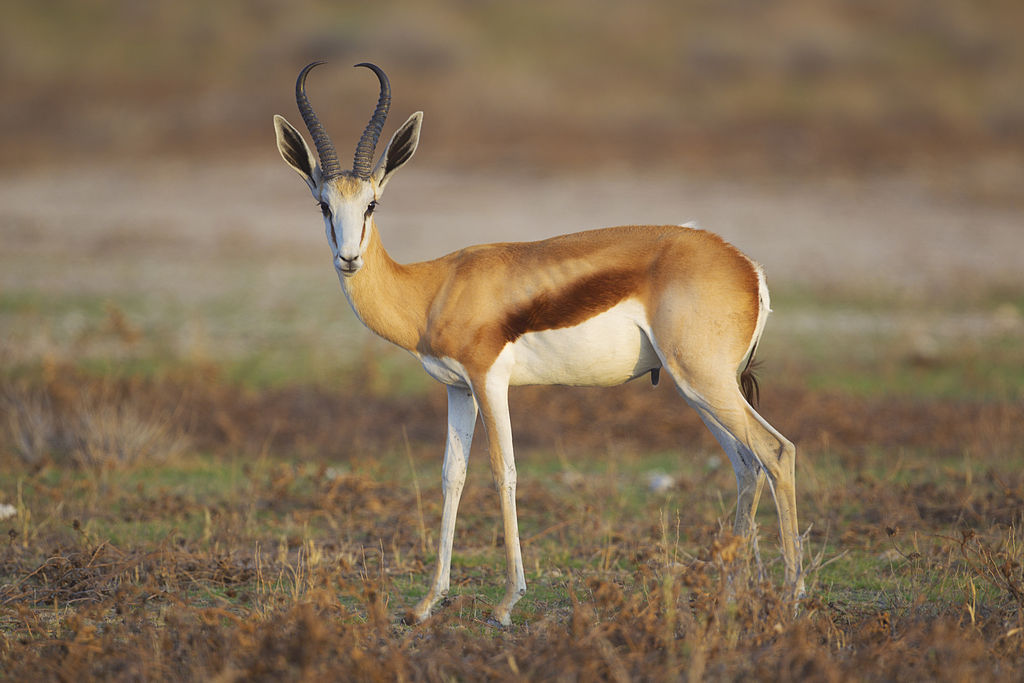
\includegraphics[width=\maxwidth{\textwidth}]{src/sample/antidorcas.jpg}
\caption{Antidorcas marsupialis, male}
\label{figure\arabic{figurecounter}}
\legend{\emph{Source}: \iftoggle{usebiblatex}{\textcite{krishnappa_adult_2012}}{\citet{krishnappa_adult_2012}}}% See: https://upload.wikimedia.org/wikipedia/commons/8/89/Antidorcas_marsupialis%2C_male_%28Etosha%2C_2012%29.jpg
\legend{\emph{Note}: Here is a note that is especially long to show what happens when it extends to more than one line.}
\end{figure}
\refstepcounter{figurecounter}
\clearpage
\section{Math examples}

This section contains some math-heavy text adapted from \iftoggle{usebiblatex}{\textcite{dwilkins1995}}{\citet{dwilkins1995}}.
In non-relativistic wave mechanics, the wave function $\psi(\mathbf{r},t)$ of a particle satisfies the Schrödinger Wave Equation
%
\begin{equation}
 i\hbar\frac{\partial \psi}{\partial t}
  = \frac{-\hbar^2}{2m} \left(
    \frac{\partial^2}{\partial x^2}
    + \frac{\partial^2}{\partial y^2}
    + \frac{\partial^2}{\partial z^2}
  \right) \psi + V \psi.
\end{equation}
%
It is customary to normalize the wave equation by
demanding that
%
\begin{equation}
\int \!\!\! \int \!\!\! \int_{\textbf{R}^3}
      \left| \psi(\mathbf{r},0) \right|^2\,dx\,dy\,dz = 1.
\end{equation}
%
A simple calculation using the Schr\"{o}dinger wave
equation shows that
%
\begin{equation}
\frac{d}{dt} \int \!\!\! \int \!\!\! \int_{\textbf{R}^3}
      \left| \psi(\mathbf{r},t) \right|^2\,dx\,dy\,dz = 0,
\end{equation}
%
and hence
%
\begin{equation}
\int \!\!\! \int \!\!\! \int_{\textbf{R}^3}
      \left| \psi(\mathbf{r},t) \right|^2\,dx\,dy\,dz = 1
\end{equation}
%
for all times~$t$. If we normalize the wave function in this
way then, for any (measurable) subset~$V$ of $\textbf{R}^3$
and time~$t$,
%
\begin{equation}
\int \!\!\! \int \!\!\! \int_V
      \left| \psi(\mathbf{r},t) \right|^2\,dx\,dy\,dz
\end{equation}
%
represents the probability that the particle is to be found
within the region~$V$ at time~$t$.

\begin{table}[h] % Table float
\caption{This caption has math characters that remain lowercase: \relax\macrocapwrap{$\psi(\mathbf{r},t)$} }
\label{table\arabic{tablecounter}}
\begin{tabu}{l c c} \\ \hline
Column1 & Column2 & Column3 \\ \hline
Row1 & 2.0 & 3.0 \\
Row2 & 2.0 & 3.0 \\
Row3 & 7.0 & 8.0 \\ \hline
\end{tabu}
\end{table}
\refstepcounter{tablecounter}
%
}{}
%%%%%%%%%%%%%%%%%%%%%%%%%%%%%%%%%%%%%%%
% Back matter
%%%%%%%%%%%%%%%%%%%%%%%%%%%%%%%%%%%%%%%
\SingleSpacing                          % Back matter should be single spaced
\AfterEndEnvironment{table}{\SingleSpacing} % Reset these environments
\AfterEndEnvironment{figure}{\SingleSpacing}
\AfterEndEnvironment{quote}{\SingleSpacing}
\AfterEndEnvironment{quotation}{\SingleSpacing}

\edef\defaulttolerance{\the\tolerance}
\tolerance 500                          % Increase tolerance to prevent material extending into margins
\hbadness 500

\iftoggle{useendnotes}{%                % If you're using endnotes, output them here
  \setsecnumdepth{none}                 % No section numbering in end notes
  \bookmarksetup{startatroot}           % Make Notes appear at root level of PDF bookmarks
  \phantomsection%                      % Need for hyperref
  \addcontentsline{toc}{chapter}{%      % Add a chapter-level heading for
    \hspace{-\cftchapterindent}%        %  Notes to the ToC
    \notesname%
  }%
  \renewcommand*{\notedivision}{%
    \chapter*{\notesname}%
  }
  \printpagenotes                       % Output the notes
  \setsecnumdepth{all}%                 % Turn section numbering back on after printing
}{}

\bookmarksetup{startatroot}
\chapter*{\bibheading}                  % In the running text, use a chapter-level heading
                                        % for the bibliography section
\phantomsection
\addcontentsline{toc}{chapter}{%        % In the TOC, add a custom chapter-level heading
  \hspace{-\cftchapterindent}%          % that will be flush against the left margin
  \bibheading%
}
%\phantomsection
%\addtocontents{toc}%                    % Add this 'mark' to TOC so subsequent pages use
%  {\protect\markboth{\bibheading}{Page}}%   the bibliography heading (unlikely since
%                                        %   the appendices follow quickly)
\iftoggle{usebiblatex}{%                % Output the bibliography
  \printbibliography[heading=none]      % Using a 'biblatex' package; do not let
                                        %   'biblatex' output a heading
}{%
  \renewcommand\bibsection{}            % Do not let 'natbib' output a heading
  \bibliographystyle{\natbibstyle}      % Using 'natbib' to print bibliography
  \bibliography{\bibfilename}
}

\appendix                               % Indicate start of appendices
                                        % Appendices are considered 'mainmatter' in this
                                        %   documentclass
\tolerance \defaulttolerance            % Set tolerance back to default
\hbadness \defaulttolerance

\addtocontents{toc}{\protect%           % Only include appendix title in table of contents
  \setcounter{tocdepth}{0}}%            %   and omit sub-headings
\renewcommand*{\chapnamefont}%          % Reset font for 'Appendix' in chapter titles
    {\normalfont\MakeTextUppercase}
\makeatletter                           % Clear page after printing appendix title
  \renewcommand{\memendofchapterhook}%
  {%
    \clearpage
    \m@mindentafterchapter
    \@afterheading
  }
\makeatother

\phantomsection                         % Need '\phantomsection' to place hyperref
                                        %   bookmark more accurately
\addcontentsline{toc}{part}{Appendix}   %~Add "Appendix" to TOC here; comment out this
                                        %   line if you're not including appendices

%\phantomsection                        %!This is the one part of the template that I
%\addtocontents{toc}%                   %   could not get to work properly. After you
%  {\protect\markboth{APPENDIX}{Page}}  %   start listing appendices in the TOC,
                                        %   subsequent TOC pages should use "APPENDIX in
                                        %   the header instead of "CHAPTER"; however,
                                        %   this code will make "APPENDIX" appear on the
                                        %   the same page that the *first* appendix
                                        %   appears on. This problem won't affect most
                                        %   people, but if it affects you, uncomment
                                        %   these lines and move them below where
                                        %   the appendices are listed. Keep moving these
                                        %   lines down and checking the output until
                                        %   the TOC headers appear correctly

%\input{appendix1}                       %~Insert your appendices here; I recommend to use
%\input{appendix2}                       %   \input rather than \include for appendices.
%\input{appendix3}% etc.                 %   All heading commands are the same as above,
                                         %   e.g., \chapter, \section, etc.
\iftoggle{sample}{%
  \chapter{This is a chapter-level heading for an appendix}

\lipsum[1]

\section{This is the first section-level heading in the appendix}

\lipsum[1]

\subsection{This is the first sub-section-level heading in the appendix}

\lipsum[1]

\subsubsection{This is the first sub-sub-section-level heading in the appendix}

\lipsum[1]

\paragraph{This is the first paragraph-level heading in the appendix}

\lipsum[1]

\subparagraph{This is the first sub-paragraph-level heading in the appendix}

\lipsum[1] %
}{}

\backmatter                             % Start back matter according to documentclass
\makeatletter                           % Do not clear page after printing title for
  \renewcommand{\memendofchapterhook}%  %   biographical sketch
  {%
    \m@mindentafterchapter
    \@afterheading
  }
\makeatother

%\biographicalsketch{%                  %~Biographical Sketch is optional
%  \input{biography}%                   %<Enter the name of the .tex file containing your
%}%                                     %   biography or omit this line and type in
                                        %   your biography here (1 paragraph)
\end{document}
